\chapter{Data\label{chap:data}}

One of the recent missions that enables remote wind measurements and serves as the data source for this thesis, is the Emirates Mars Mission (EMM), which was launched in 2020 and entered Mars orbit in 2021. The mission is equipped with three scientific instruments: the Emirates Mars InfraRed Spectrometer (EMIRS), the Emirates Mars Ultraviolet Spectrometer (EMUS), and the Emirates eXploration Imager (EXI)\cite{Amiri2022}.

\section{Relevance}

Among the various instruments and techniques available for atmospheric measurements from orbit, high-resolution images in ultraviolet wavelengths, such as those captured by the Emirates Mars Mission's EXI\cite{Jones2021}, are particularly valuable for tracking cloud movement, which is indicative of wind patterns. 
On Mars, the very low temperatures and pressures typically cause clouds to form as water ice. However, Martian clouds can also contain CO2 and display a wide range of properties and formations\cite{clancyetalChapter052017}. While visual observation of CO2 clouds is challenging, as they are mostly formed during the polar night, water ice clouds are more easily observed and are categorized into three broad regimes: the aphelion cloud belt (see Figure 2.1), polar hoods, and high-altitude haze (see Figure 2.2). The first two categories represent clouds in the lower atmosphere, below 40 km in altitude, while the third category is found at slightly higher altitudes, above 30–40 km\cite{clancyetalChapter052017}.
\FloatBarrier
\begin{figure}[h!] 
    \centering
    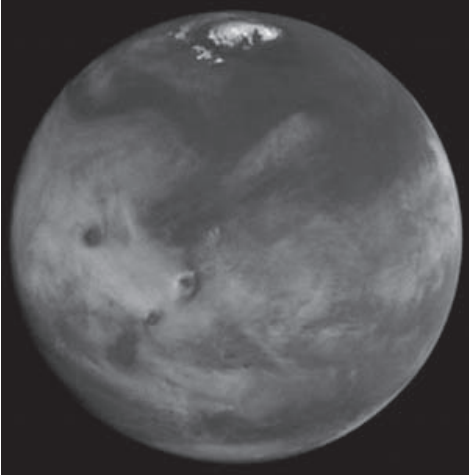
\includegraphics[width=0.5\textwidth]{fig_02.png}
    \caption{Hubble Space Telescope imagery capturing the Aphelion Cloud Belt on Mars\cite{clancyetalChapter052017}.}
\end{figure}
\FloatBarrier
\begin{figure}[h!] 
    \centering
    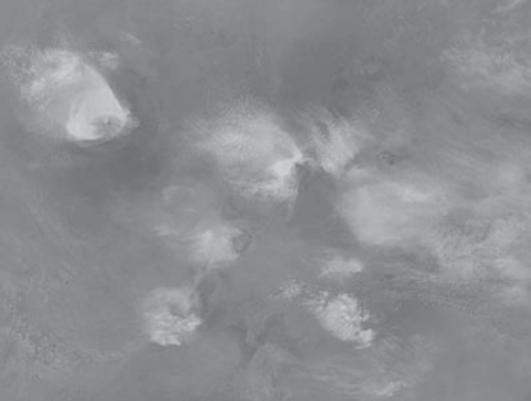
\includegraphics[width=0.5\textwidth]{fig_03.png}
    \caption{Typical afternoon cloud formations over Tharsis Montes during the northern summer (Ls = 122.3°)\cite{clancyetalChapter052017}.}
\end{figure}
\FloatBarrier
Since objective A of the Emirates Mars Mission focuses on characterizing the Martian lower atmosphere, the Emirates eXploration Imager (EXI) provides images that effectively display the altitudes where clouds are found\cite{Amiri2022}. An overview of Mars atmospheric layers mapped to EMM objectives can be seen in Figure 2.3. 
\FloatBarrier
\begin{figure}[h!] 
    \centering
    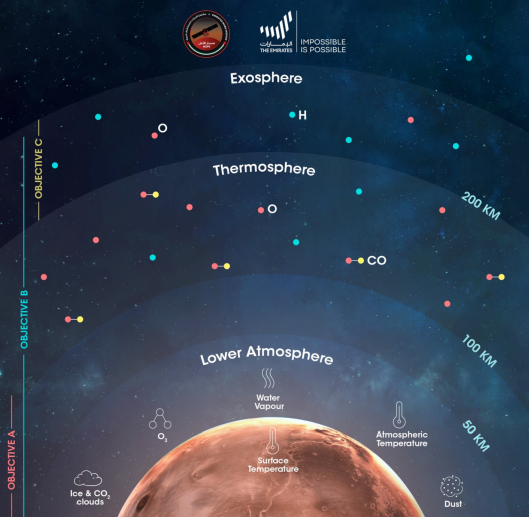
\includegraphics[width=0.8\textwidth]{fig_04.png}
    \caption{Illustration of Mars atmospheric layers mapped to EMM objectives and measurements\cite{Almatroushi2021}.}
\end{figure}
\FloatBarrier
EXI captures images across six bandpasses, centered at 220, 260, 320, 437, 546, and 635 nm, using two telescopes—one for ultraviolet (UV) and the other for visible (VIS) wavelengths, supporting different aspects of the mission's overall strategy. The full-disk images have a resolution of 2-4 km per pixel\cite{Jones2021}.

EXI’s ultraviolet imagery at 320nm is particularly well-suited for cloud tracking due to its focus on water ice optical depth. Water ice clouds have distinct absorption features in this UV spectrum, making them visible in the resulting images. Surface materials, however, do not reflect UV light at this wavelength. Consequently, any visible features, except for surface ice, are attributed to the lower atmosphere. This allows for a high degree of confidence in distinguishing atmospheric features in the UV images.

\section{Format}

The image sequences are provided in the form of FITS (Flexible Image Transport System) files, a format developed in the 1970s for archiving and exchanging astronomical data\cite{NasaFITS}. FITS files are designed to store data sets that include multidimensional arrays and two-dimensional tables. The data is organized in Header and Data Units (HDUs), which allow access to both the header containing general information and the data itself. The initial HDU is known as the Primary HDU. 
The chosen FITS files contain all data within the primary HDU. The data shape varies based on the number of images in each sequence, ranging from (6, 2880, 5760) to (22, 2880, 5760), where the first dimension indicates the number of images, and the second and third dimensions represent the height and width of the images. An illustration of the FITS file structure containing 6 images is shown in Figure 2.4. While the images are split between two bandpasses, only the images from the 320 nm bandpass were extracted for this thesis. 
\FloatBarrier
\begin{figure}[h!] 
    \centering
    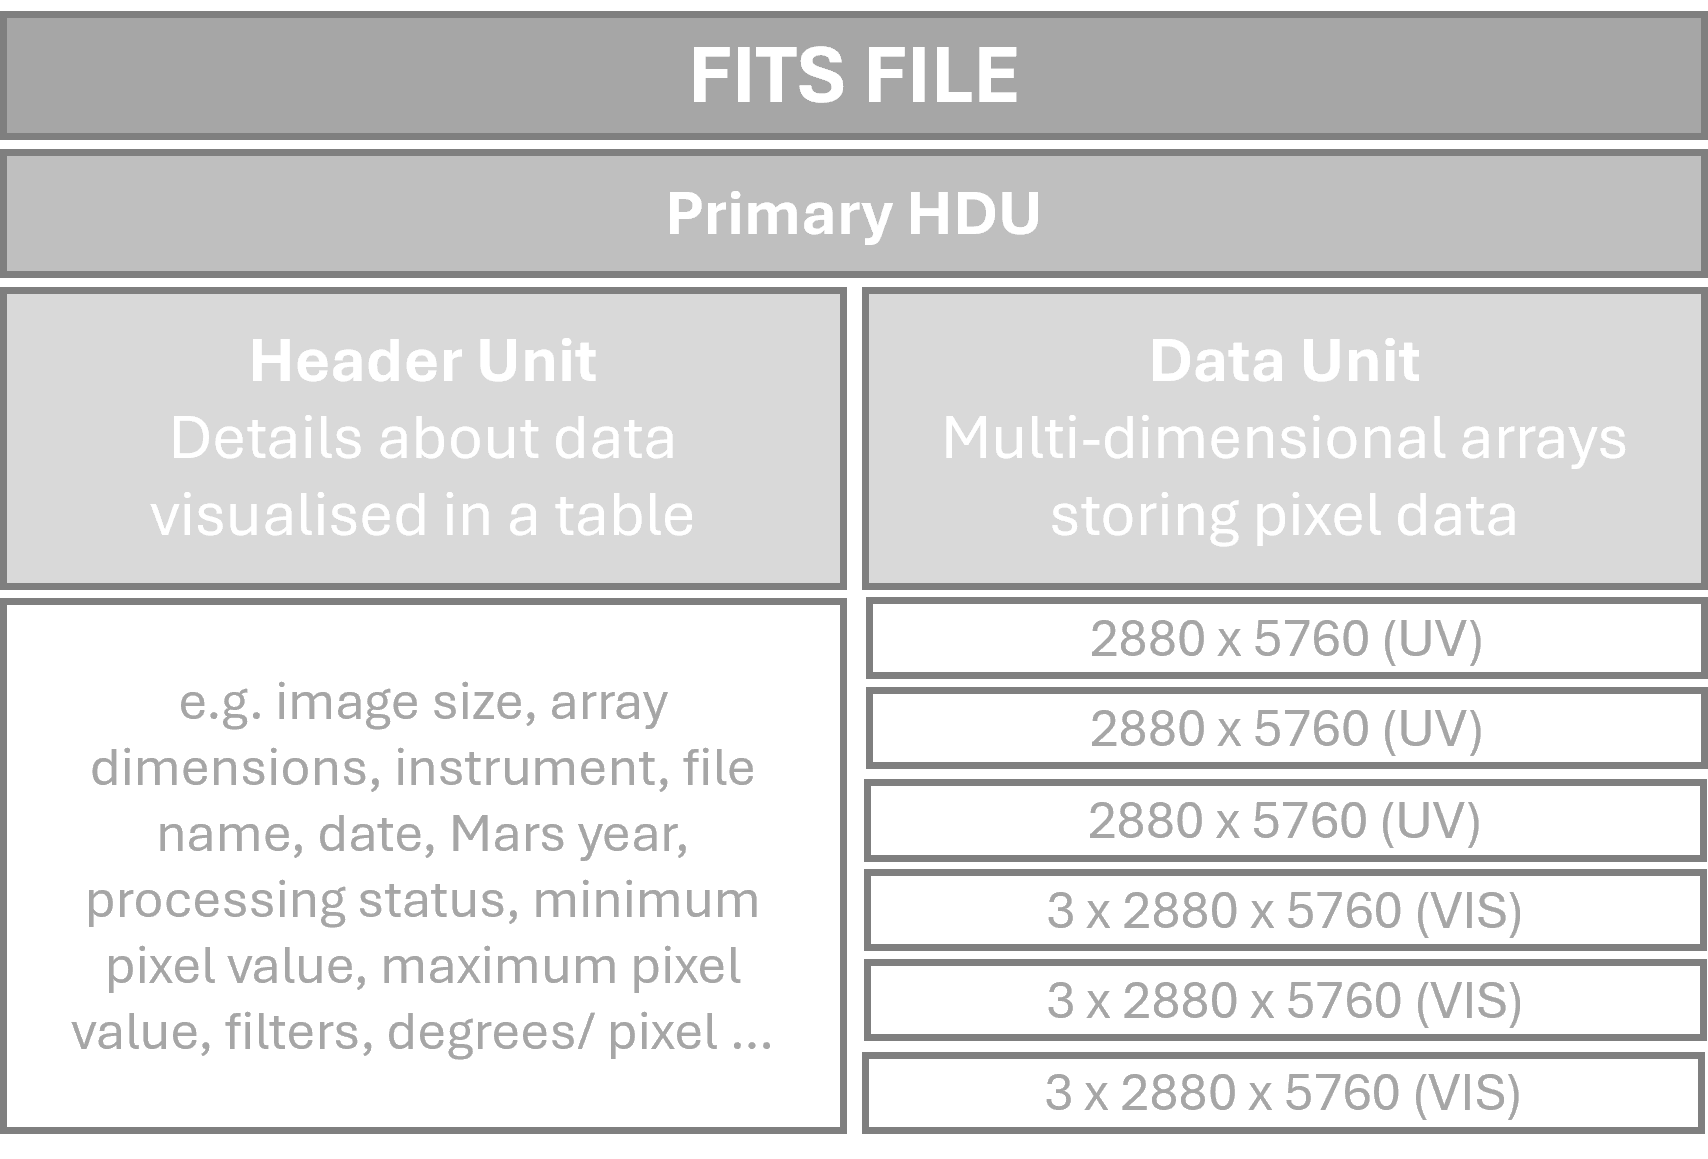
\includegraphics[width=0.8\textwidth]{fig_05.png}
    \caption{Visualization of a FITS file structure example including three visible (VIS) and three ultraviolet (UV) images.}
\end{figure}
\FloatBarrier
\section{Selection}

Among the available observation modes ranging from XOS1 to XOS14, the chosen image sequence is from XOS7 (EXI Observation Set 7). Additionally, the EXI data pipeline includes several product stages: L1 data (raw images), L2A (calibrated), L2B (map-projected), and L3 (retrievals)\cite{Jeppesen2021}. 

In a 2023 thesis by Shaimaa Ahmed AlBlooki, using UV imagery from the EXI instrument, it was identified that a jitter error (random motion) negatively impacted the accuracy of cloud tracking\cite{AlBlooki2023} (see Figure 2.5). This thesis utilizes recently released file versions, containing pointing corrected data, to mitigate jitter and improve precision of the cloud tracking.
\FloatBarrier
\begin{figure}[h!] 
    \centering
    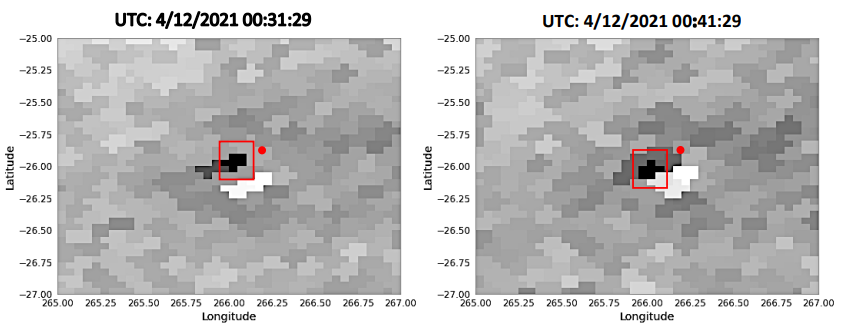
\includegraphics[width=1\textwidth]{fig_06.png}
    \caption{Example of jitter effect in older file version: EXI 635 nm XOS7 image, UTC: 4/12/2021 00:31:29-00:41:29\cite{AlBlooki2023}. The dot indicates the center of the frame. The images display a noticeable shift in crater positions.}
\end{figure}
\FloatBarrier
The selected image data set (Table 2.1) was captured during the northern summer solstice, within the solar longitude range of 131° to 146°. This period captures the aphelion cloud belt, characterized by its non-uniform cloud distribution (approx.14-50 km altitude) that begins forming around LS = 0°, reaches maximum optical depth around LS = 80°, and starts dissipating around LS = 140°. Typically, this cloud belt becomes longitudinally continuous by approximately LS = 60° and maintains this continuity until about LS = 140°, aligning with the solar latitudes of the chosen images\cite{clancyetalChapter052017}. 
\FloatBarrier
\begin{table}[h!]
    \centering
    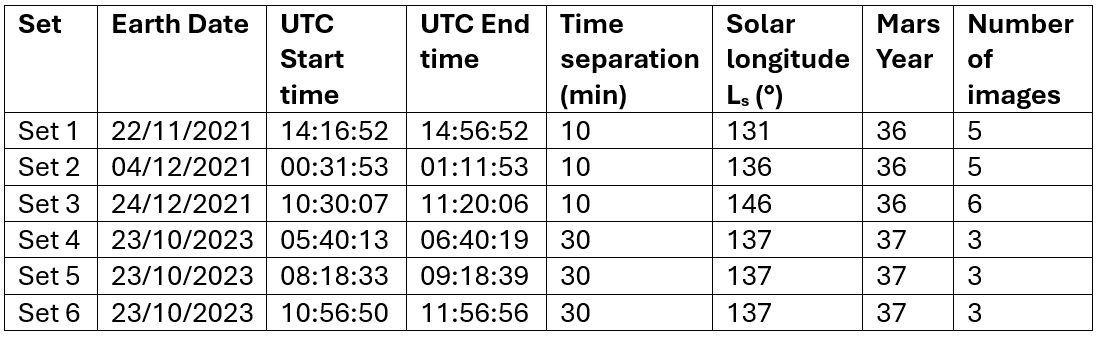
\includegraphics[width=1\textwidth]{table_01.png}
    \caption{List of set of images used in this thesis.}
\end{table}
\FloatBarrier
Shortly after the EXI mission began delivering data, images were captured at 5-minute intervals. In later sequences, the time separation increased to 30 minutes. While Sets 1, 2, and 3, captured in 2021 soon after data delivery commenced, were available with 5-minute intervals, the sequences used in this thesis were extracted at 10-minute intervals. This adjustment resulted in fewer images but was made to ensure higher accuracy in the cloud tracking process. Furthermore, the purpose of using the first three sequences is to enable comparison with results from an earlier thesis that used the same images, albeit without pointing correction\cite{AlBlooki2023}. The last three sets evaluate image sequences from 2023, providing a comparison two years later at a different time interval.
\FloatBarrier
\begin{figure}[h!] 
    \centering
    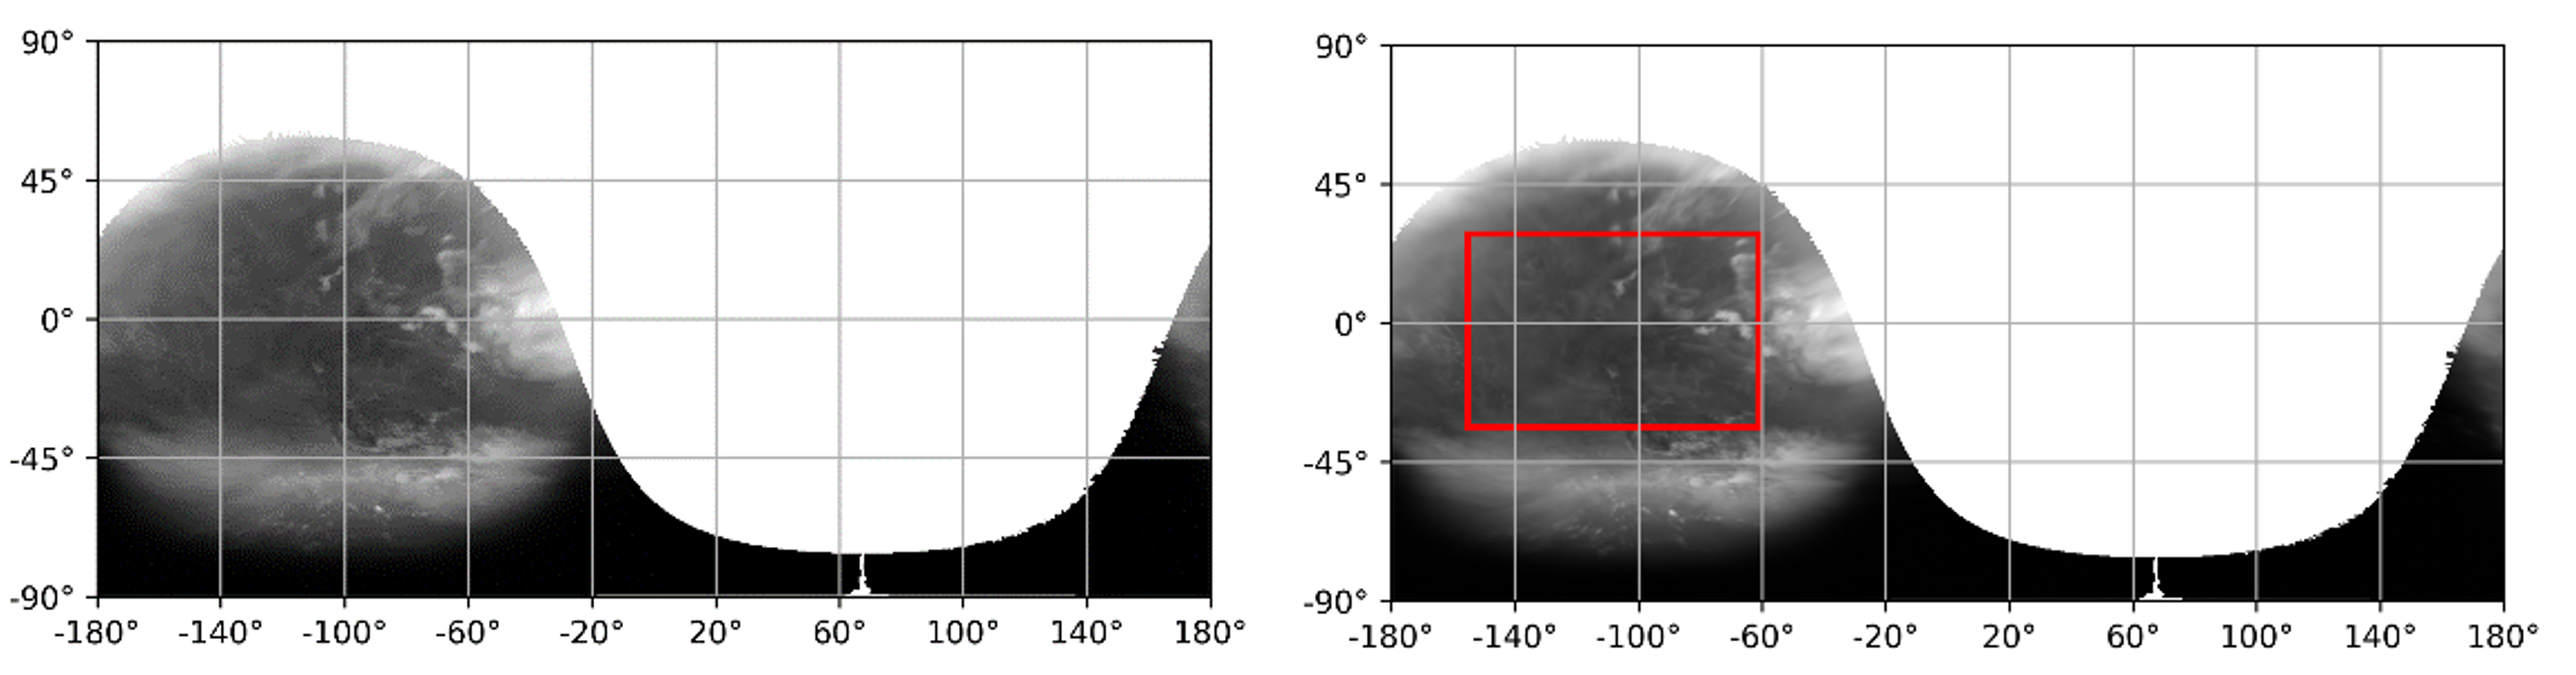
\includegraphics[width=1\textwidth]{fig_07.png}
    \caption{Example visualisation of the cropped area in images - UTC: 24/12/2021 10:30:07}
\end{figure}
\FloatBarrier
The images were cropped (see Figure 2.6) consistently across each sequence to exclude highly distorted areas at the edges of the hemisphere and regions that are not illuminated by the Sun. 
The resulting cropped regions cover longitudes from -167.5° to -23.75° and latitudes from -33.75° to 35°. An overview of these cropped regions is presented in Figure 2.7, and Table 2.2 details the latitude and longitude boundaries.
\FloatBarrier
\begin{figure}[h!] 
    \centering
    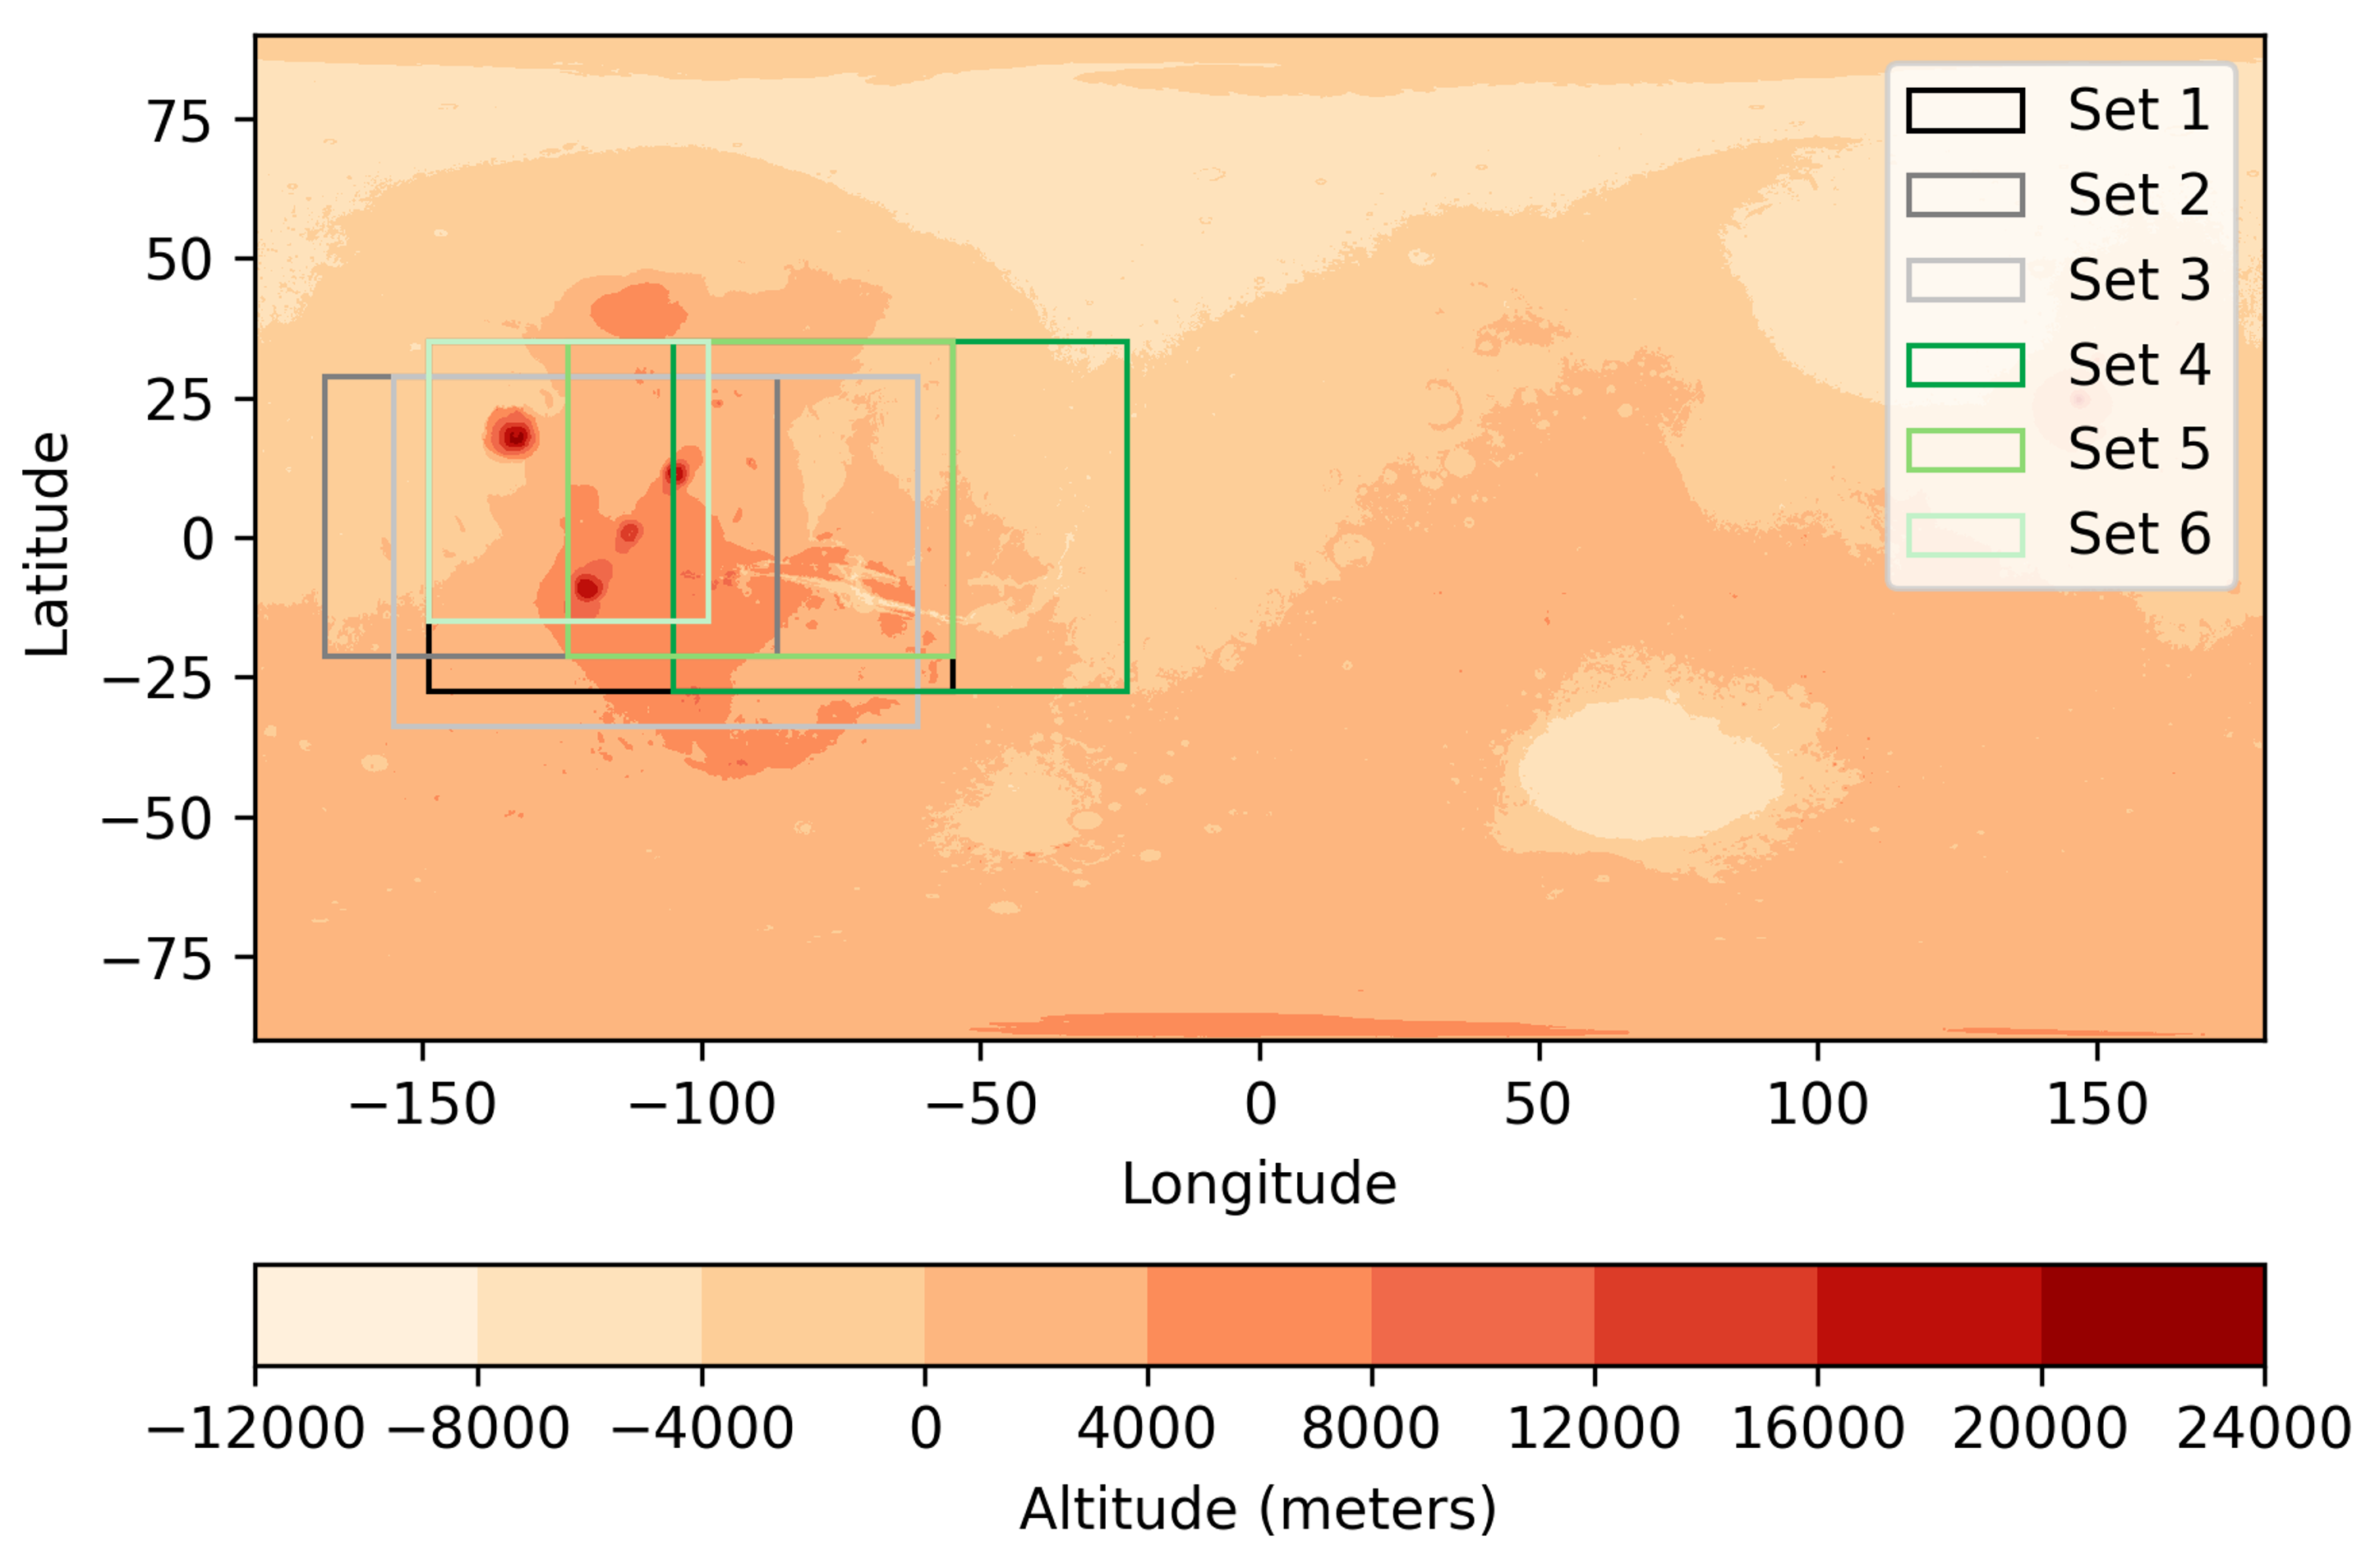
\includegraphics[width=1\textwidth]{fig_08.png}
    \caption{Illustration of the six areas of study using Mars Orbiter Laser Altimeter (MOLA) topography data\cite{MOLA}, where the red shades represent the topography of Mars and the frames indicate the cropped area for each image sequence.}
\end{figure}
\FloatBarrier
\begin{table}[h!]
    \centering
    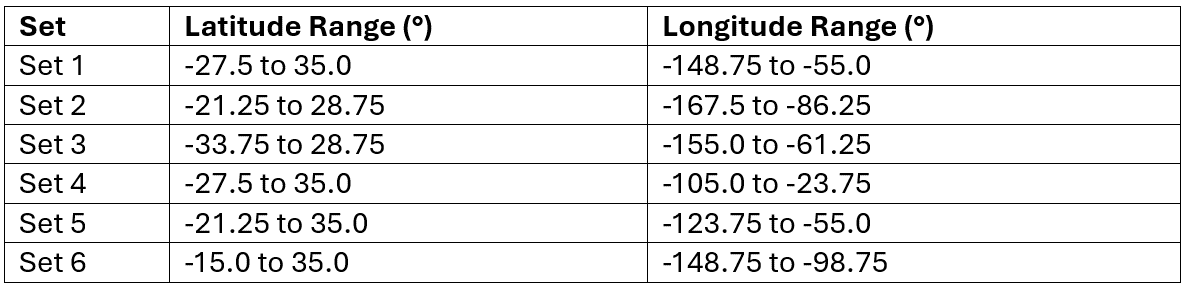
\includegraphics[width=1\textwidth]{table_02.png}
    \caption{ List of image sets cropped latitude and longitude ranges.}
\end{table}
\FloatBarrier
\section{Exploration}

The original projected UV images have a resolution of 2880 pixels in height and 5760 pixels in width, resulting in a total of 16.588.800 pixels. Of these, approximately 55 percent are NaN values, which represent areas not corresponding to Martian terrain. The remaining non-NaN pixels display a broad range of intensities, averaging between -24 and 3.930. The average intensity is approximately 819, with a median of 724 and a standard deviation of 796. The kurtosis and skewness of the pixel intensities are on average 0.08 and 0.79.
\FloatBarrier
\begin{figure}[h!] 
    \centering
    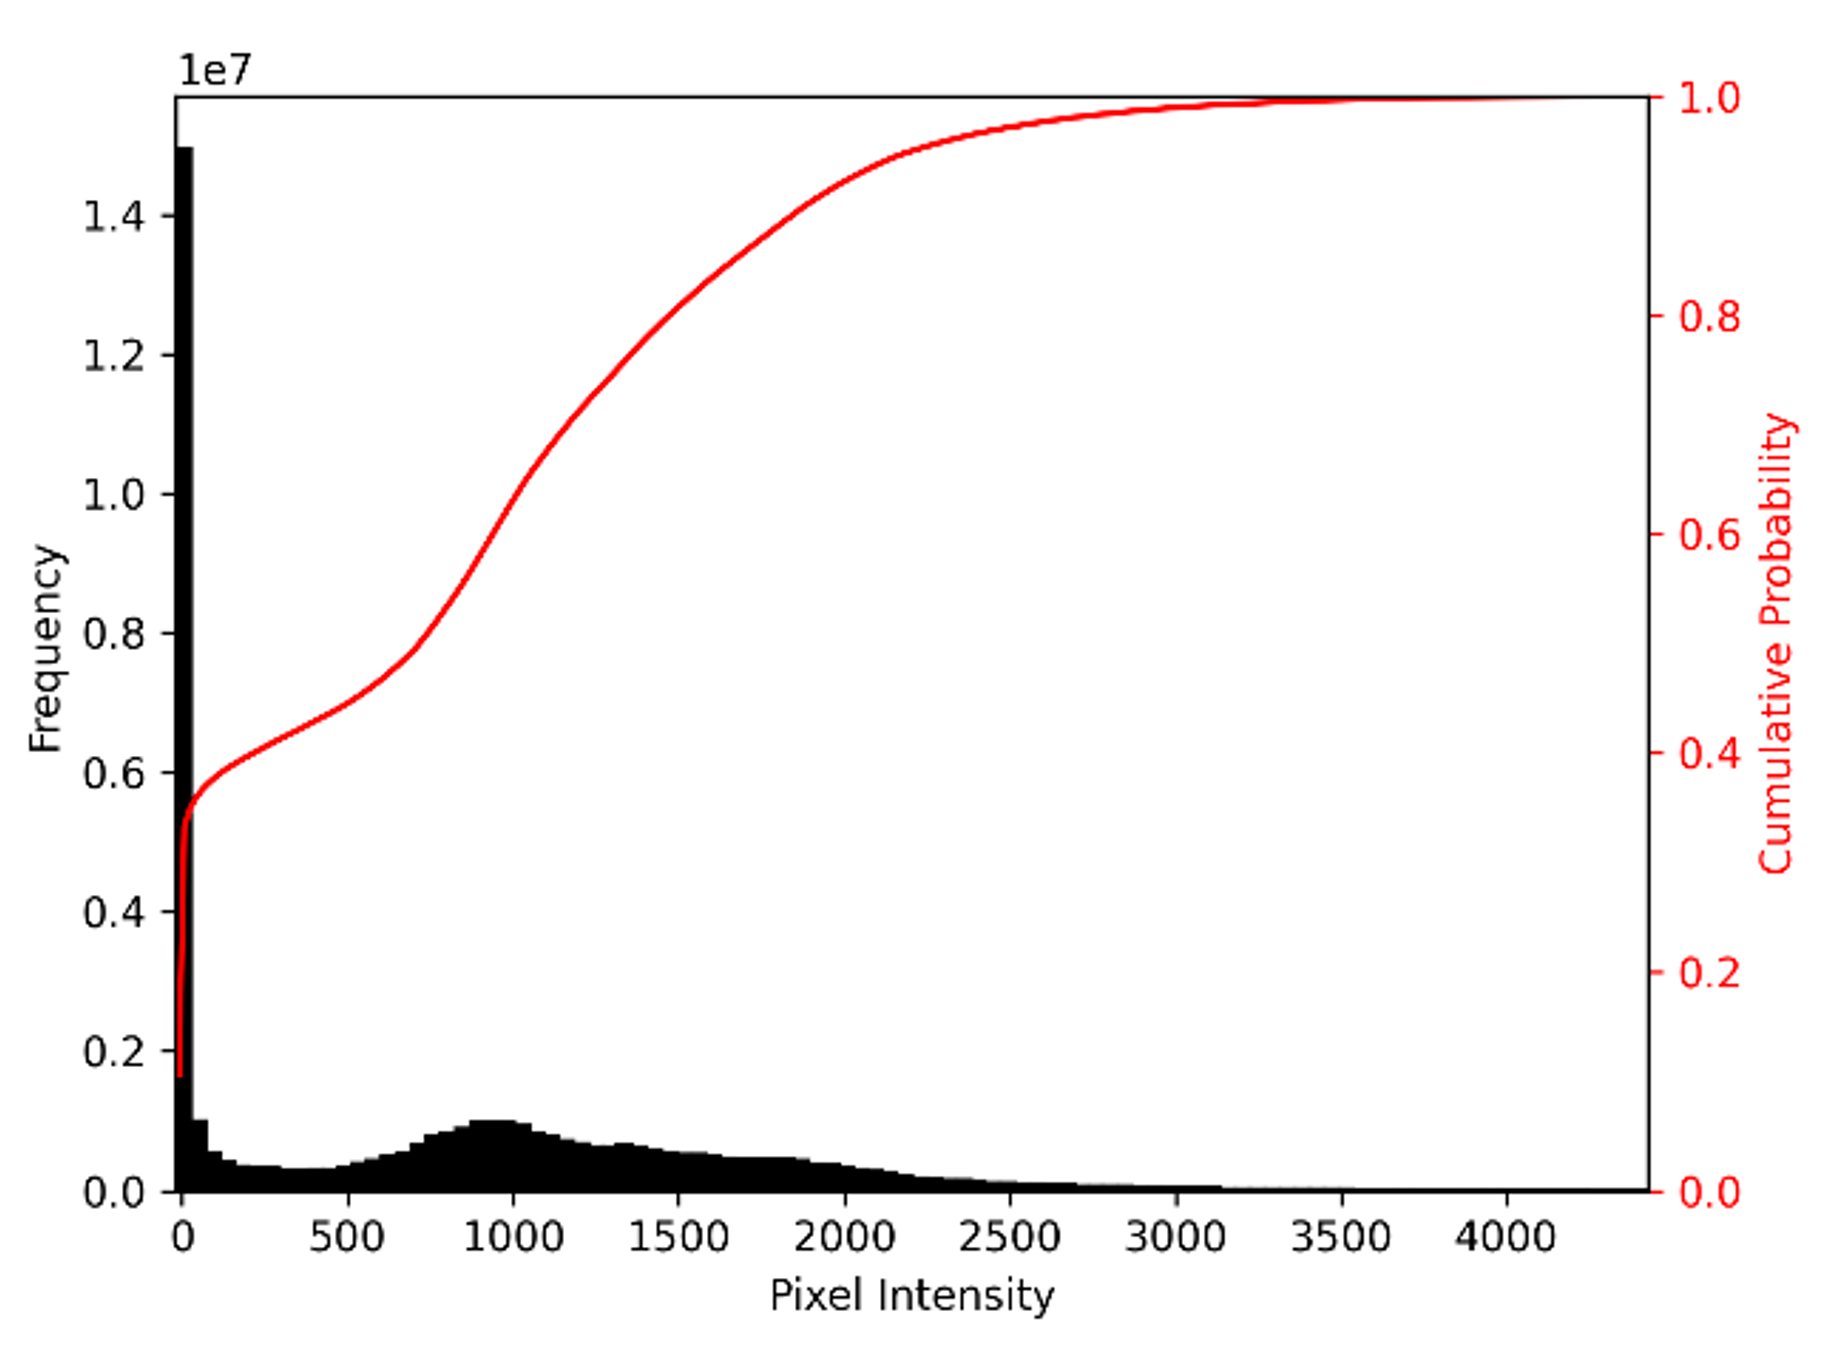
\includegraphics[width=0.8\textwidth]{fig_09.png}
    \caption{Visualization of the histogram and cumulative distribution of all selected image data across image sequences.}
\end{figure}
\FloatBarrier
Analysing the histogram and cumulative distribution function, shown in Figure 2.8, reveals that a significant proportion of pixel intensities are concentrated in the low range. Additionally, there is a noticeable peak in the lower-to-mid range of intensities, while higher intensity values are relatively sparse.

When reading the images back in Python, the “io.imread“ function from the “scikit-image” package normalized the pixel values to a range between 0 and 1, ensuring better readability in the subsequent analysis. The underlying equation for normalization is as follows:

\begin{equation}
\text{x}_{\text{normalized}} = \frac{x - x_{\text{min}}}{x_{\text{max}} - x_{\text{min}}}
\end{equation}

Where \( x_{\text{min}} \) represents the minimum intensity and \( x_{\text{max}} \) represents the maximum intensity of the image pixel data.
\FloatBarrier
\begin{figure}[h!] 
    \centering
    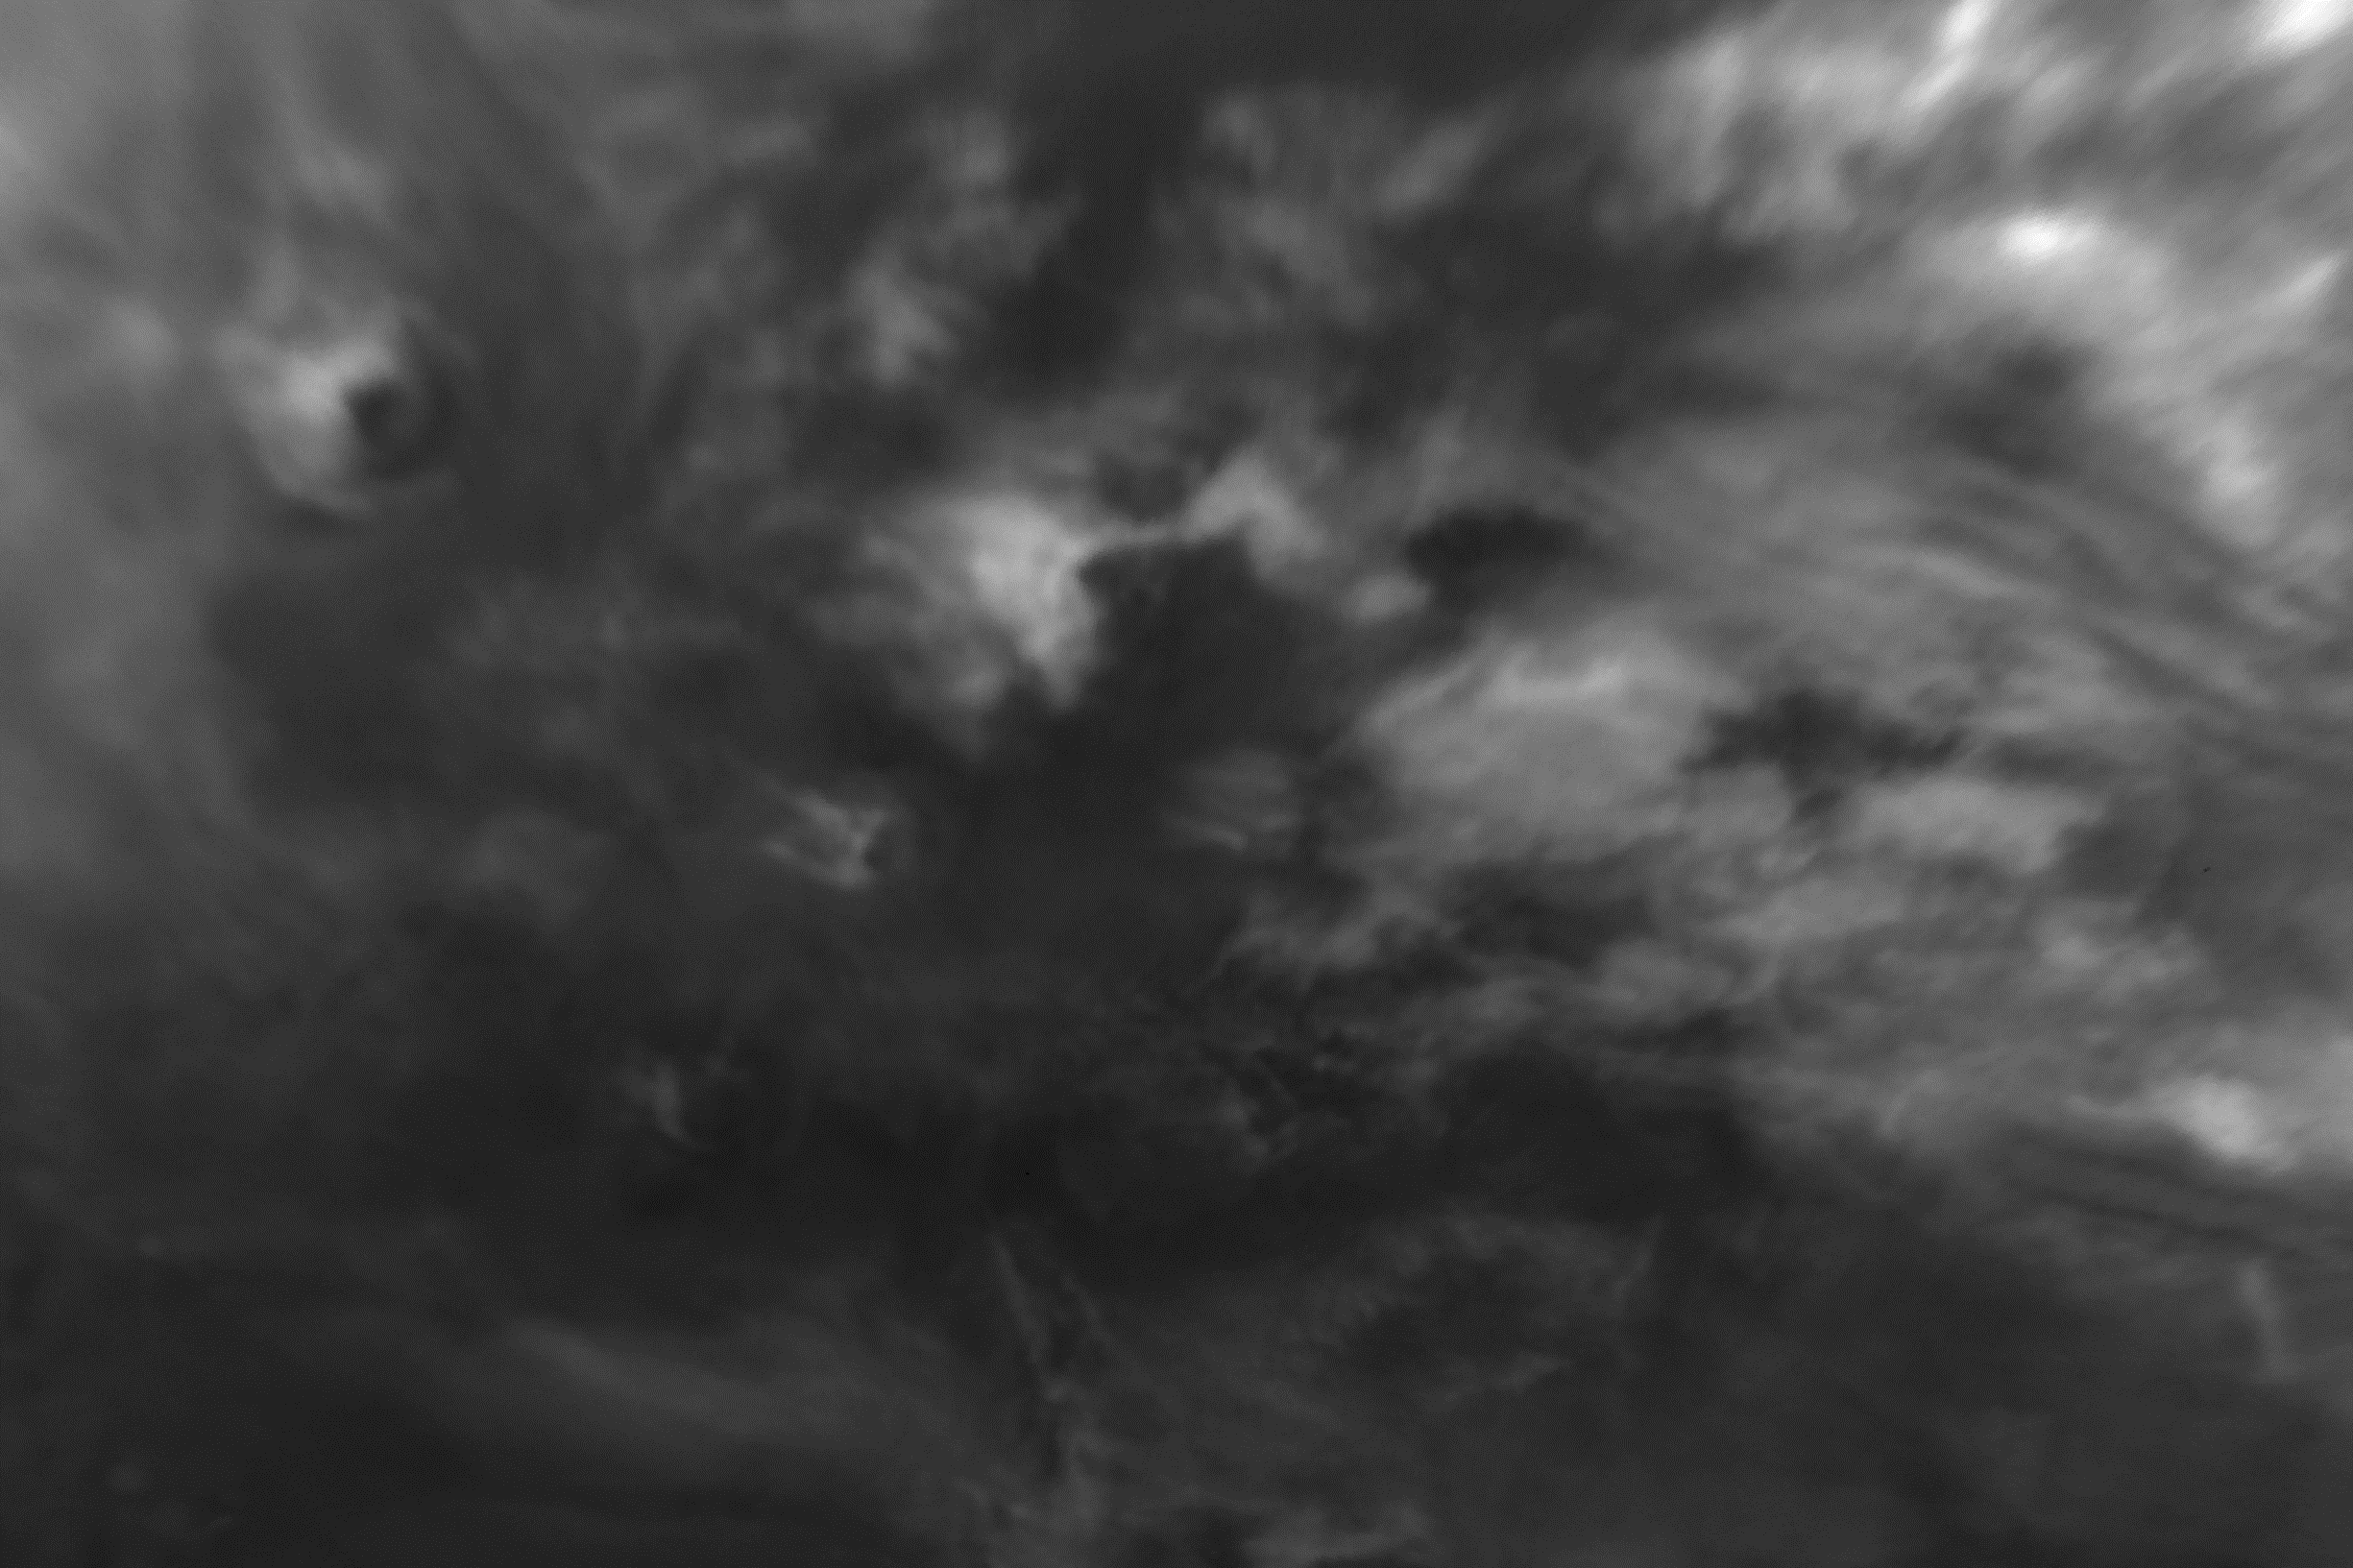
\includegraphics[width=0.8\textwidth]{fig_10.png}
    \caption{First cropped image in set 1 - UTC: 22/11/2021 14:16:52 (Latitude: -27.5° to 35.0°, Longitude: -148.75° to -55.0°), range in kilometers: approx. 5546 x 3697}
\end{figure}
\FloatBarrier
\begin{figure}[h!]
    \centering
    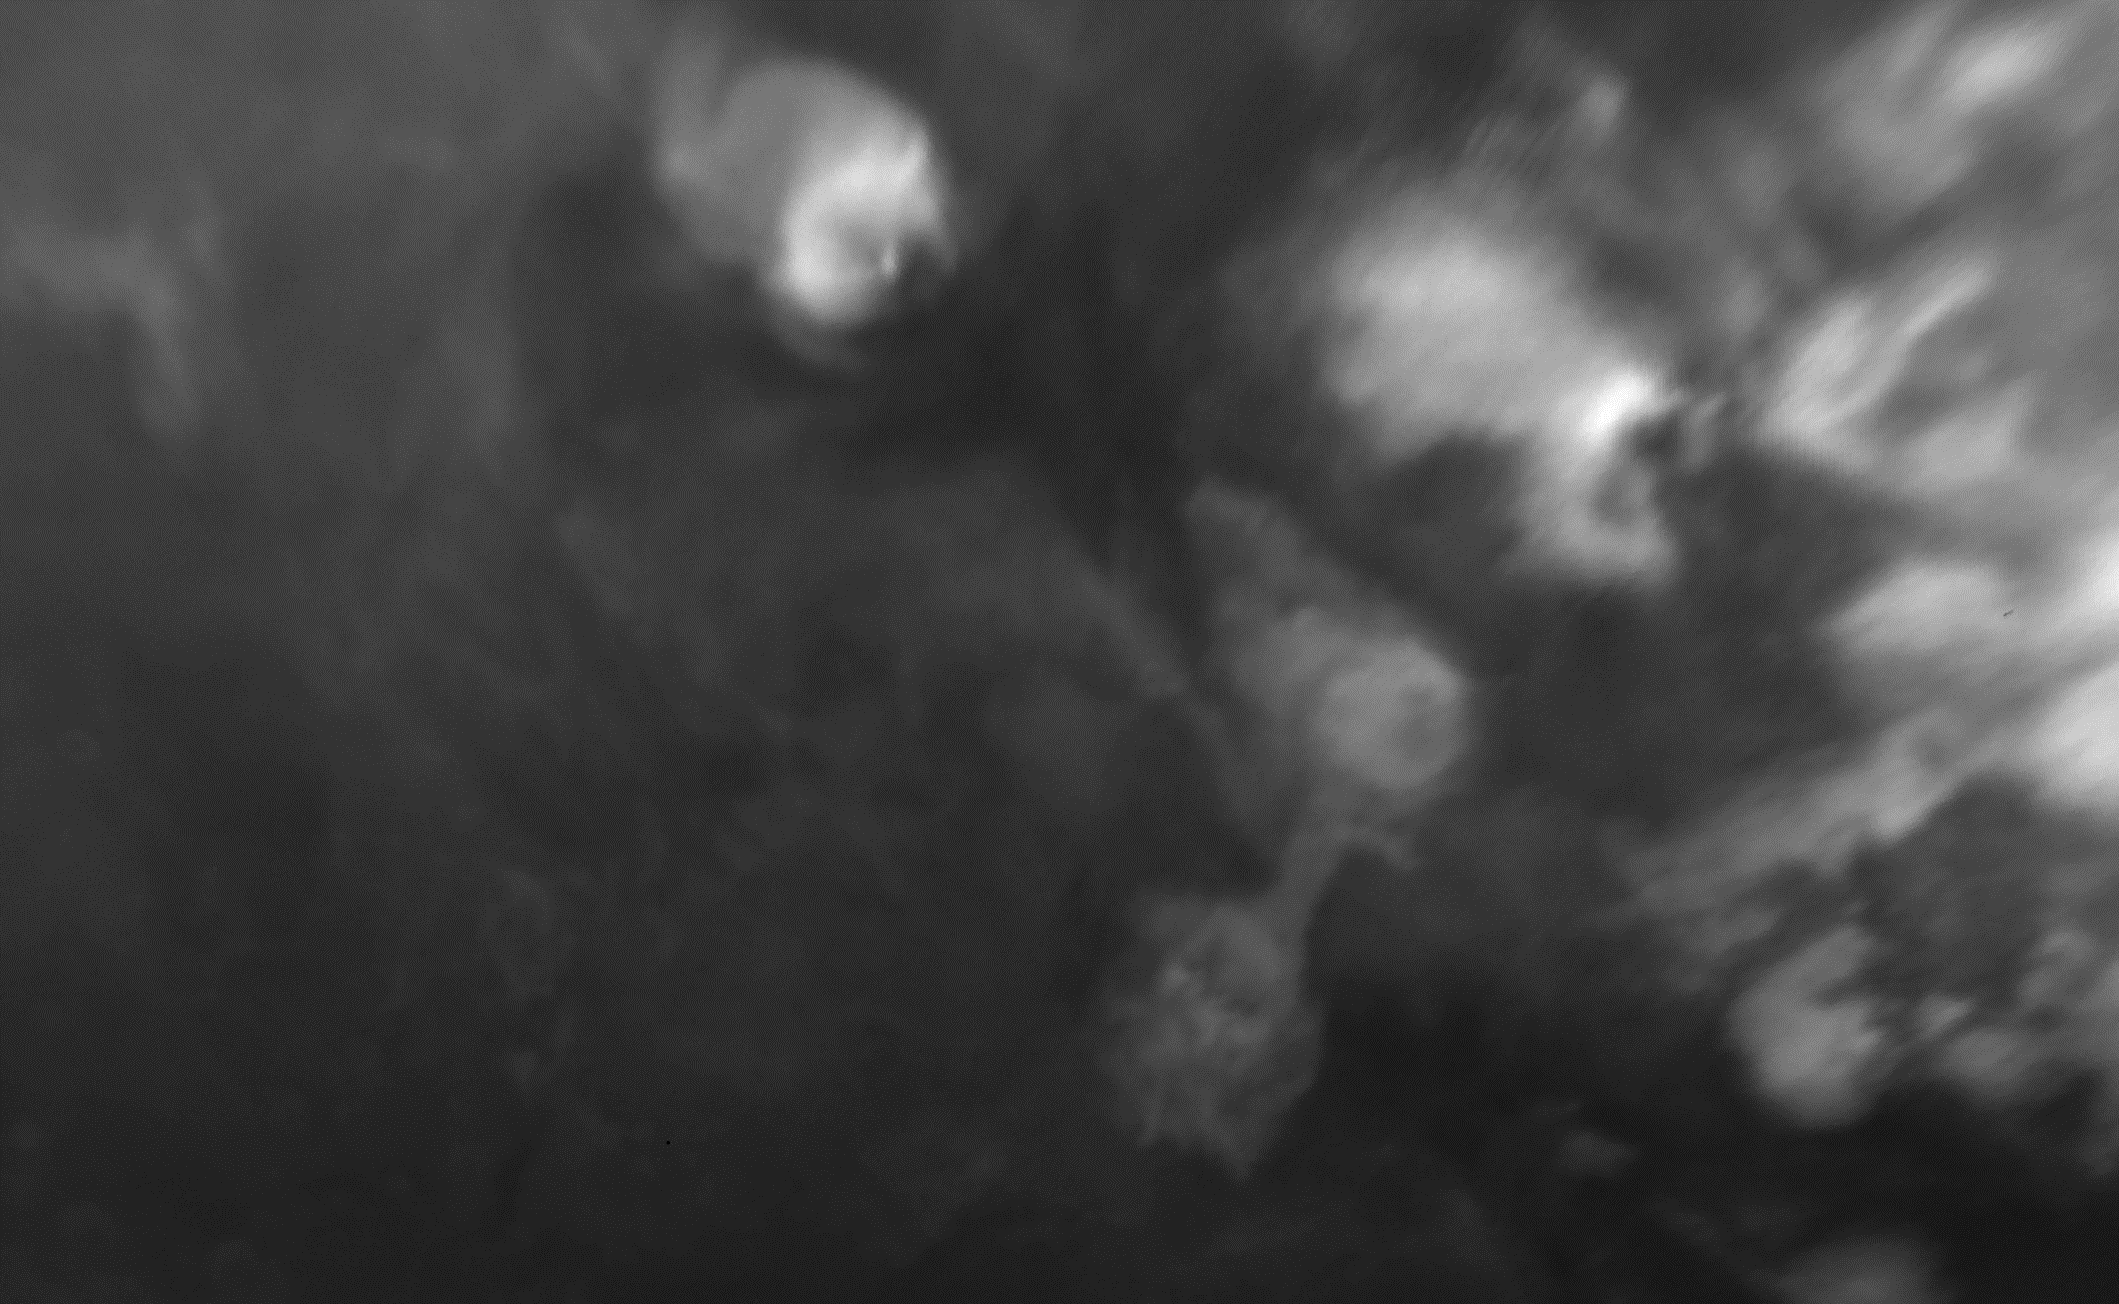
\includegraphics[width=0.8\textwidth]{fig_11.png}
    \caption{First cropped image in set 2 - UTC: 04/12/2021 00:31:53 (Latitude: -21.25° to 28.75°, Longitude: -167.5° to -86.25°), range in kilometers: approx. 4807 x 2958}
\end{figure}
\FloatBarrier
\begin{figure}[h!]
    \centering
    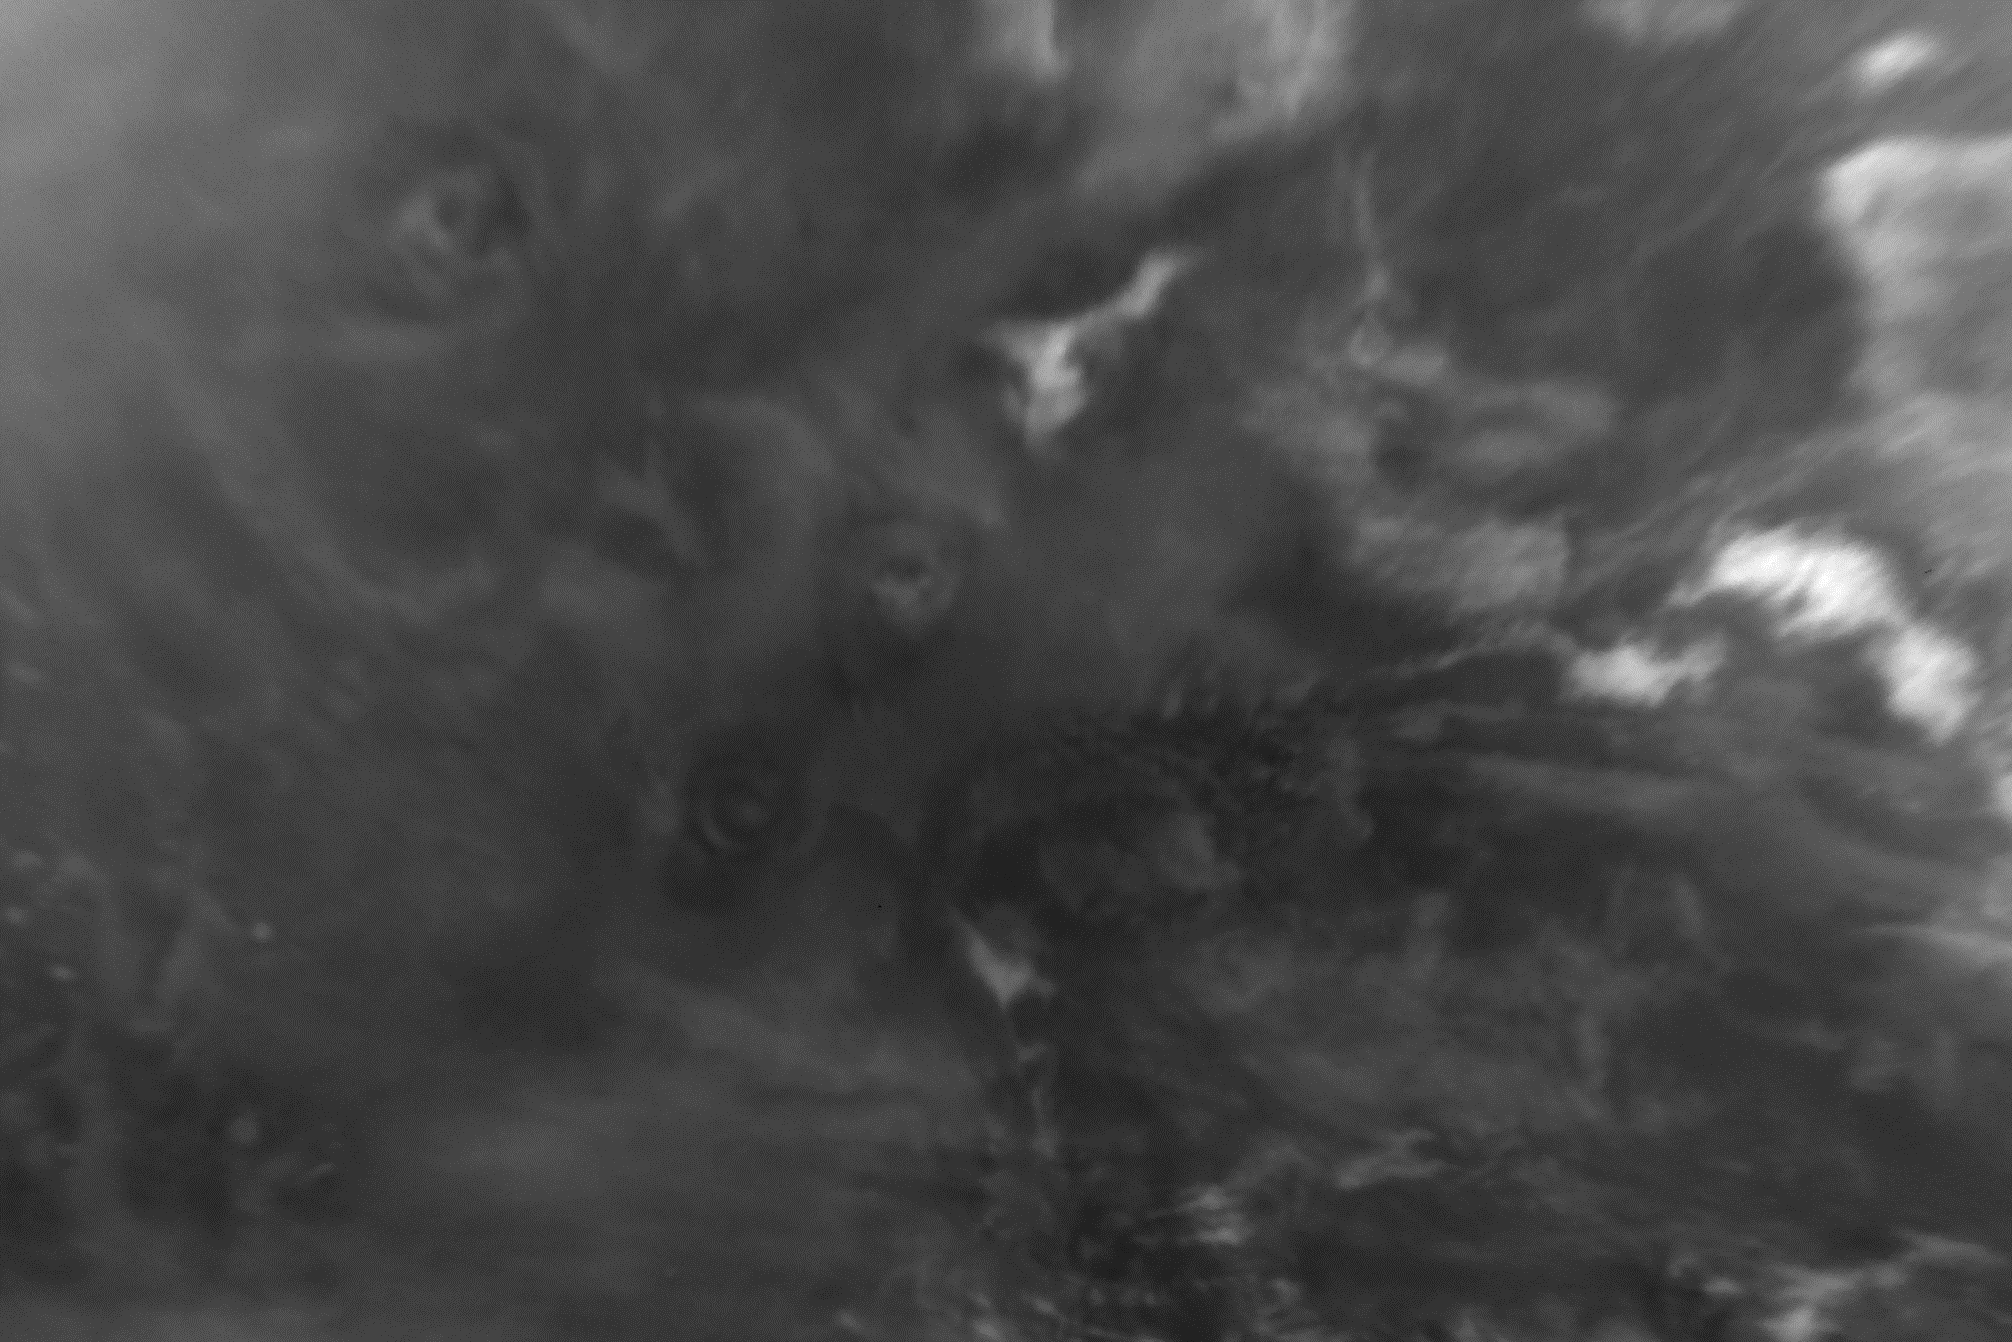
\includegraphics[width=0.8\textwidth]{fig_12.png}
    \caption{First cropped image in set 3 - UTC: 24/12/2021 10:30:07 (Latitude: -33.75° to 28.75°, Longitude: -155.0° to -61.25°), range in kilometers: approx. 5546 x 3697}
\end{figure}
\FloatBarrier
\begin{figure}[h!]
    \centering
    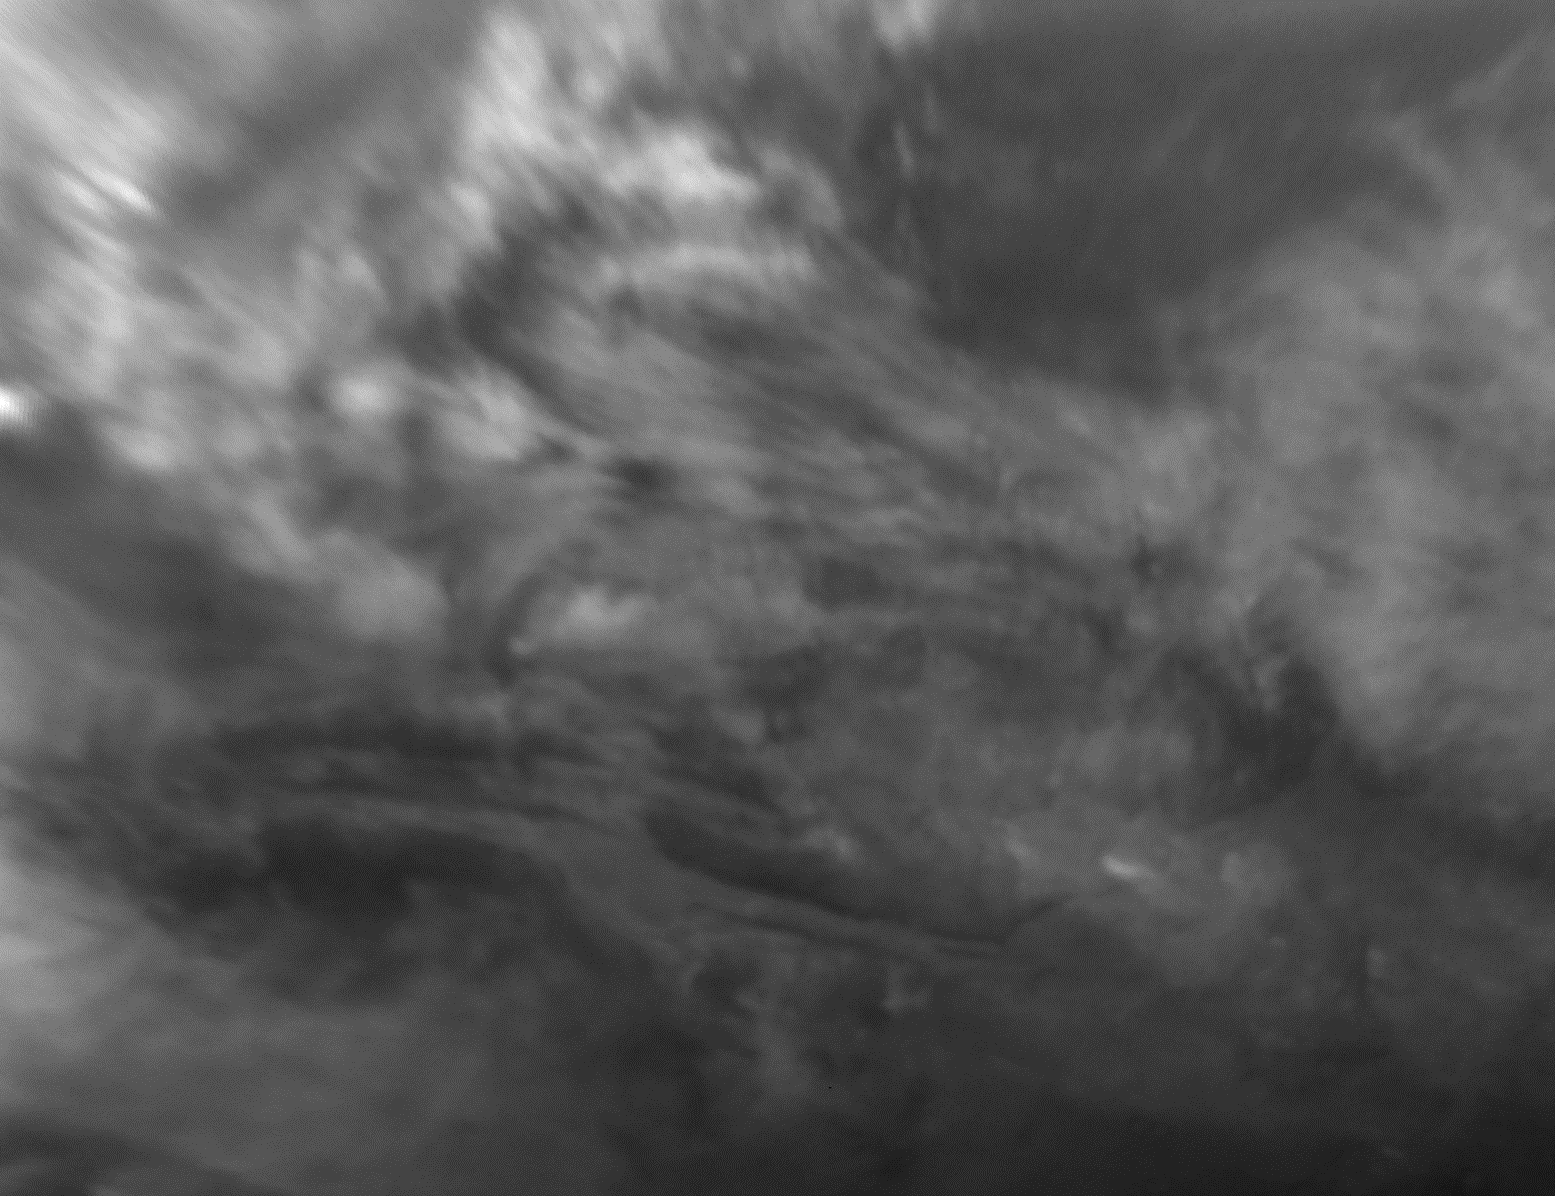
\includegraphics[width=0.6\textwidth]{fig_13.png}
    \caption{First cropped image in set 4 - UTC: 23/10/2023 05:40:13 (Latitude: -27.5° to 35.0°, Longitude: -105.0° to -23.75°), range in kilometers: approx. 4807 x 3697}
\end{figure}
\FloatBarrier
\begin{figure}[h!]
    \centering
    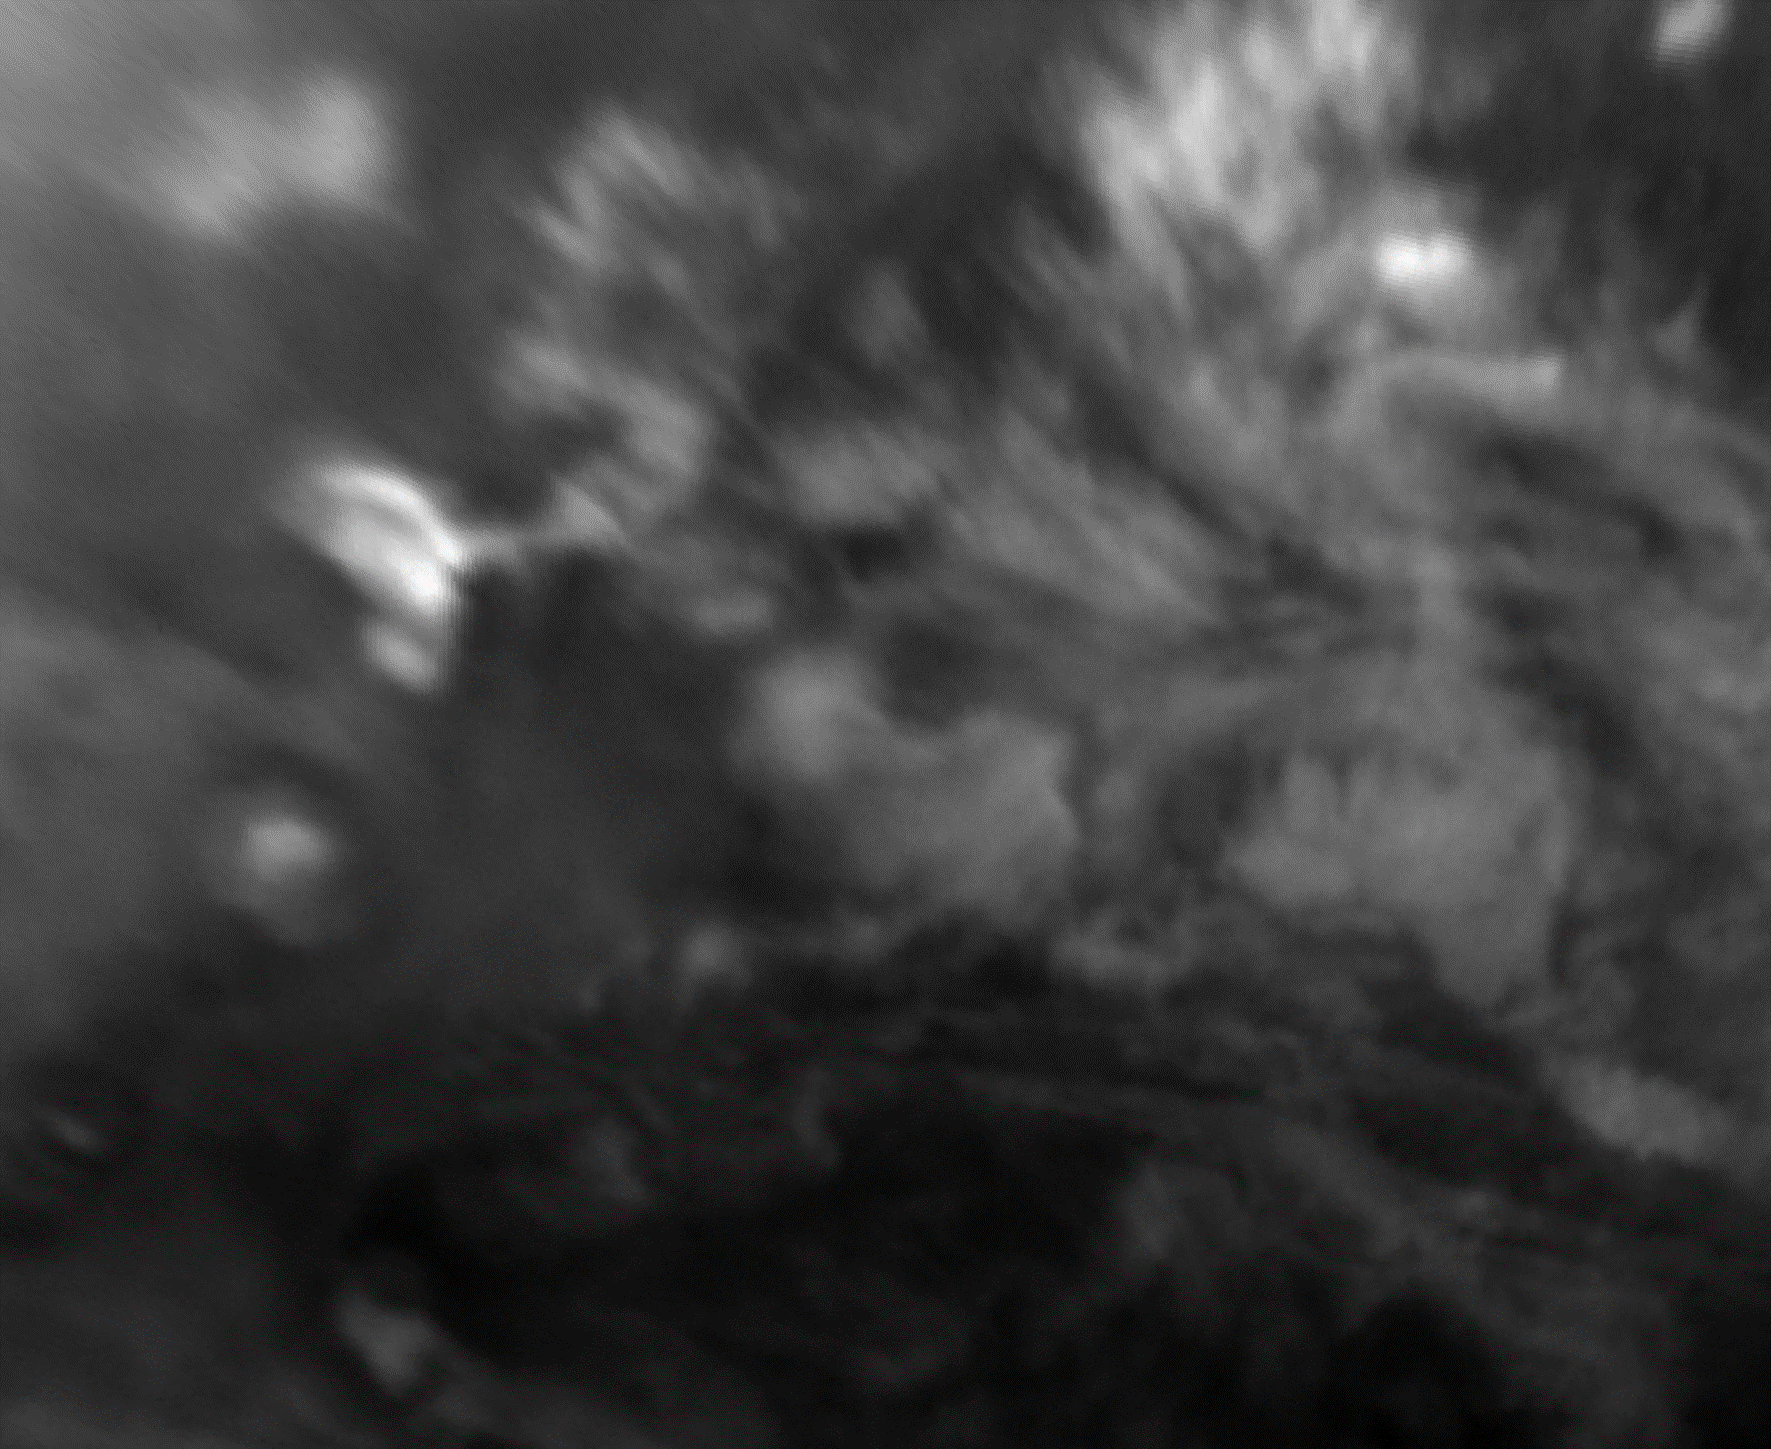
\includegraphics[width=0.6\textwidth]{fig_14.png}
    \caption{First cropped image in set 5 - UTC: 23/10/2023 08:18:33 (Latitude: -21.25° to 35.0°, Longitude: -123.75° to -55.0°), range in kilometers: approx. 4067 x 3328}
\end{figure}
\FloatBarrier
\begin{figure}[h!]
    \centering
    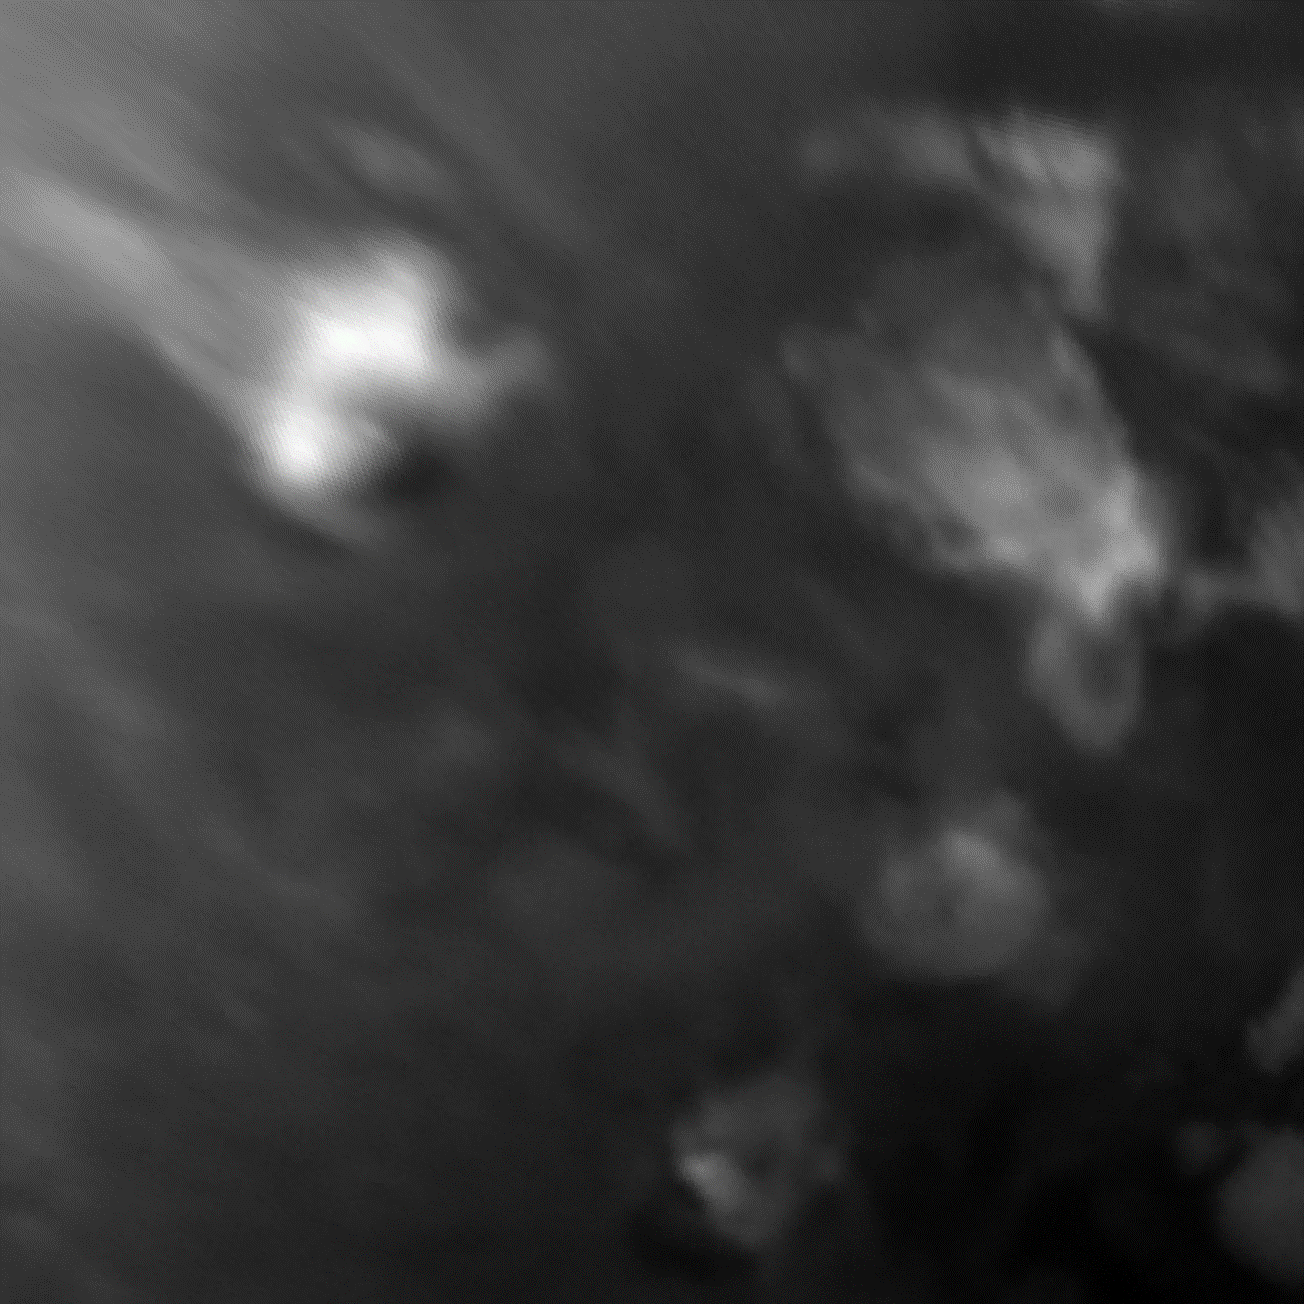
\includegraphics[width=0.6\textwidth]{fig_15.png}
    \caption{First cropped image in set 6 - UTC: 23/10/2023 10:56:50 (Latitude: -15.0° to 35.0°, Longitude: -148.75° to -98.75°), range in kilometers: approx. 2958 x 2958}
\end{figure}
\FloatBarrier
An overview of the first images from each sequence is displayed in Figures 2.9 through 2.14.
Based on visual observation, the images appear quite dark. This darkness may result from various factors, such as the scarcity of clouds in darker areas, differences in solar illumination, and the presence of cloud shadows.
There are noticeable brightness inconsistencies within the sequences and the clouds are spread out over larger regions with occasional brighter hot-spots. 
\FloatBarrier
\begin{figure}[h!]
    \centering
    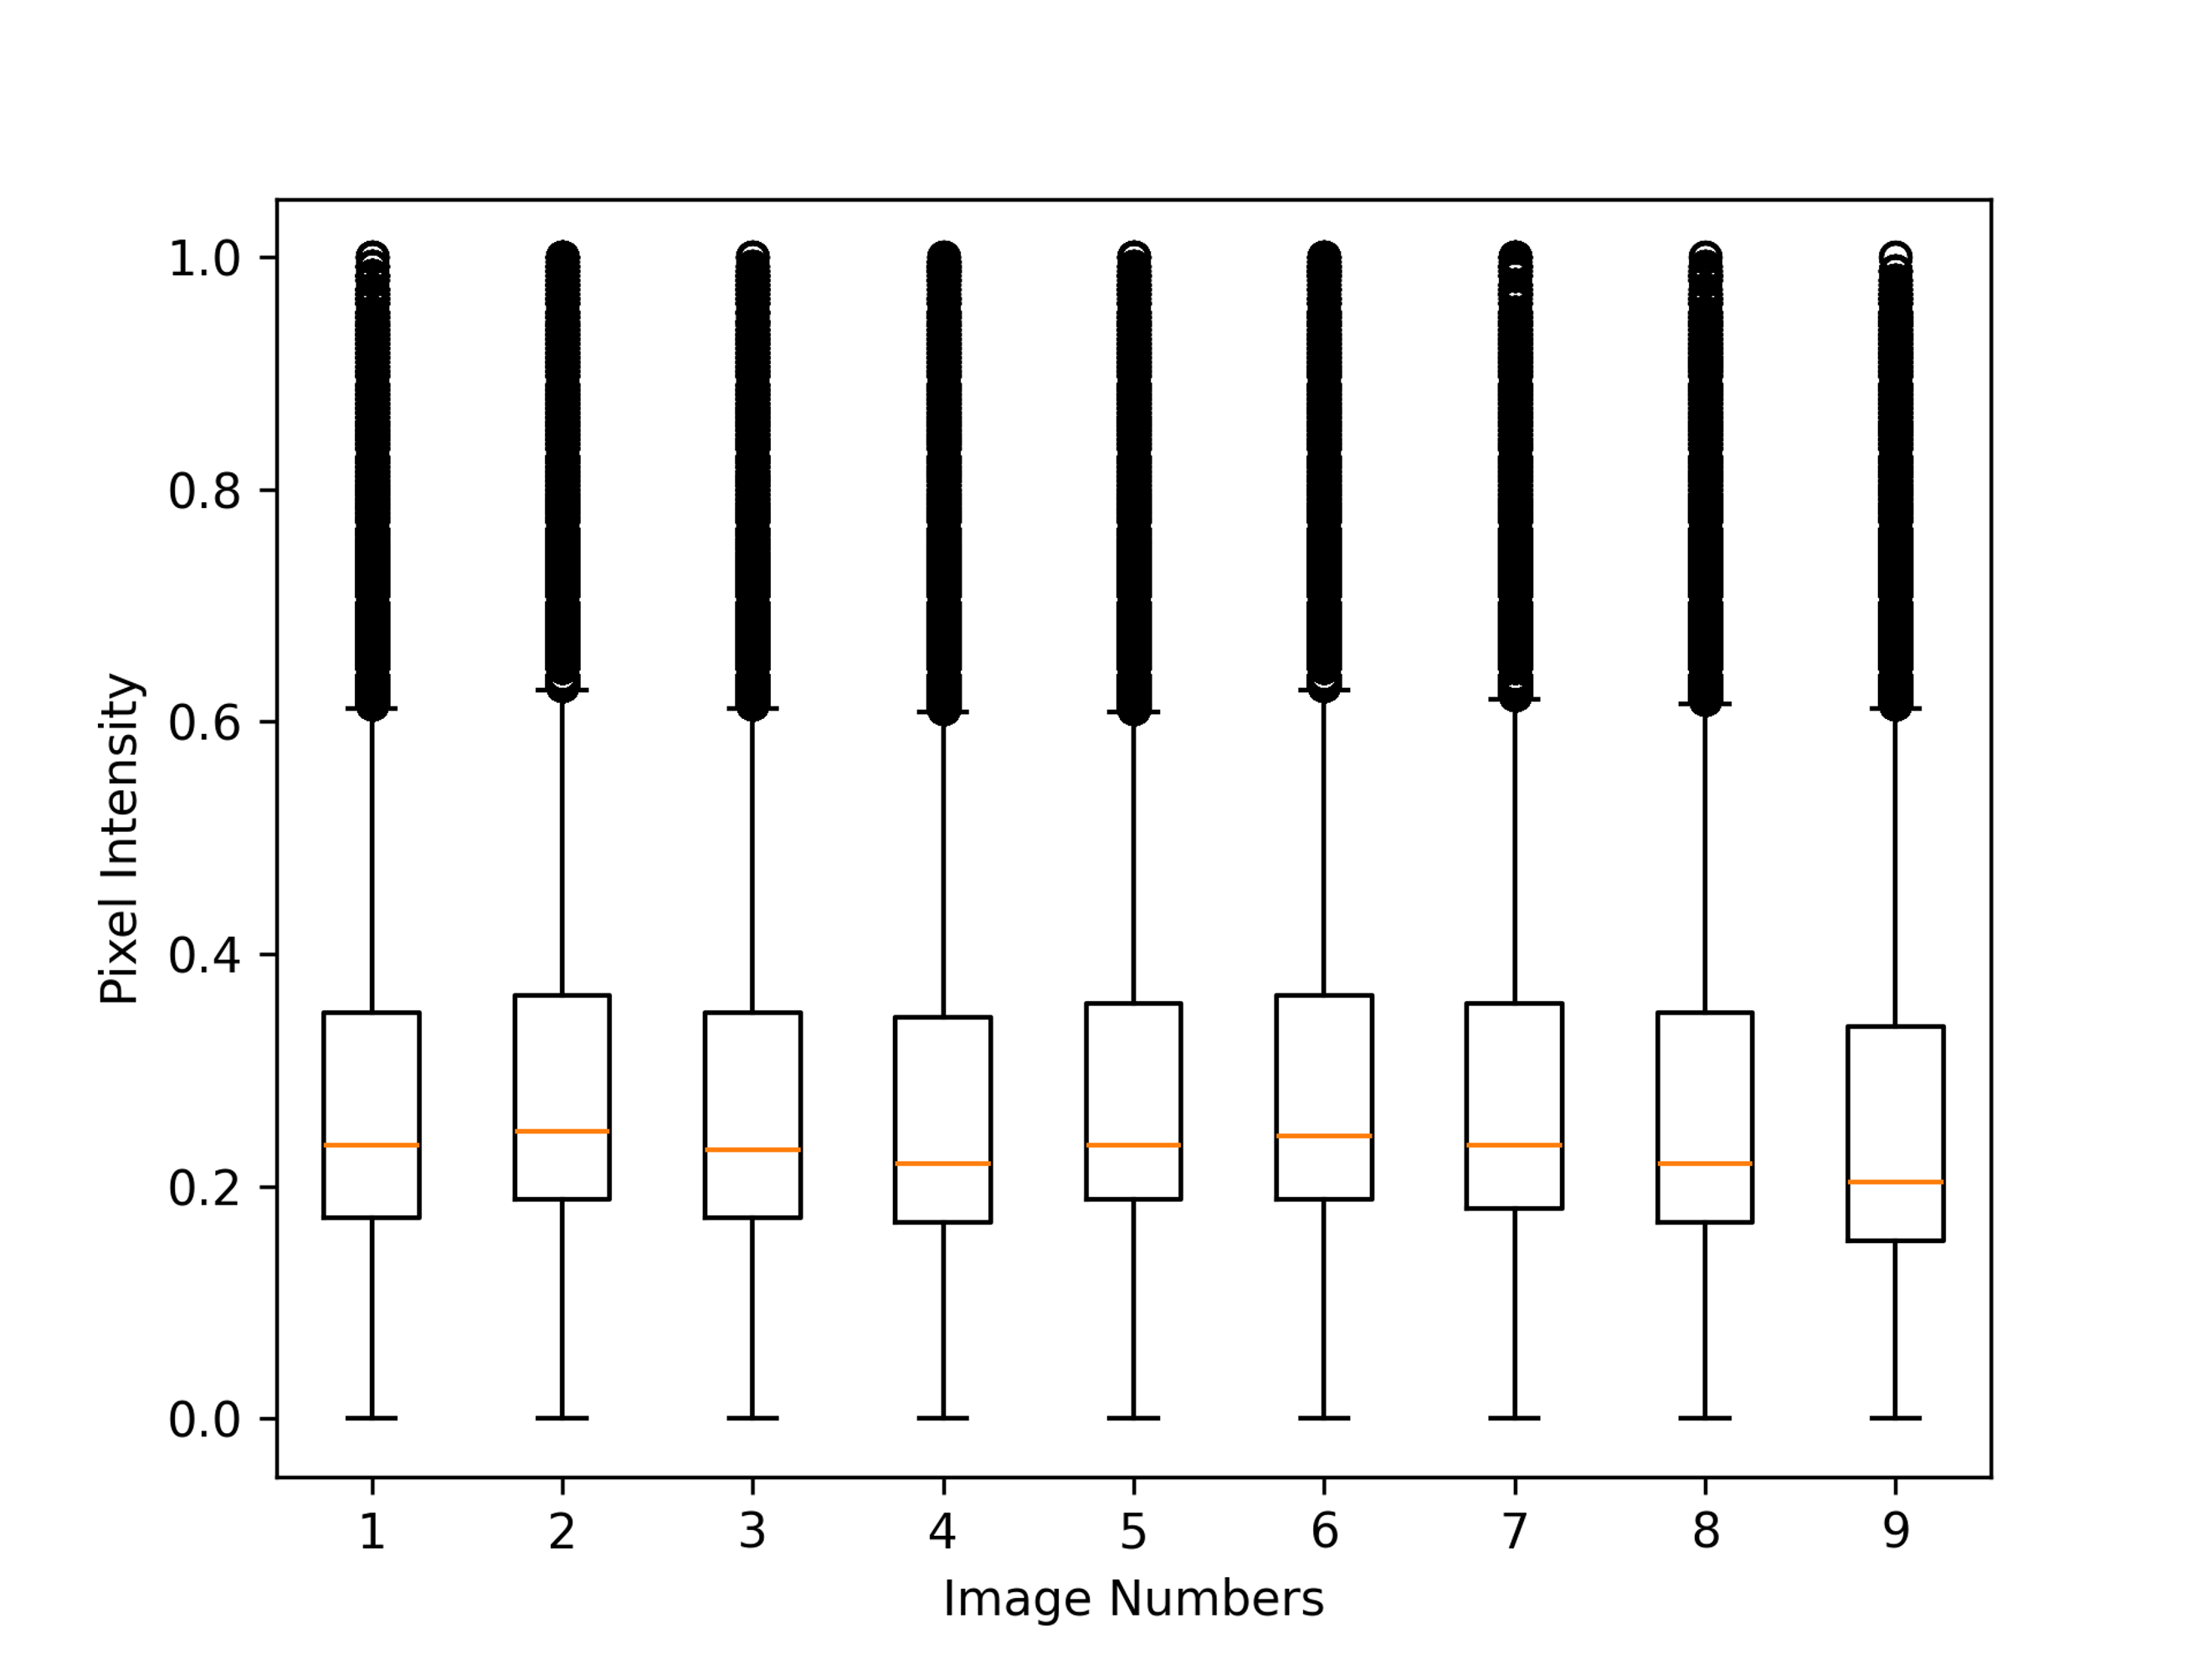
\includegraphics[width=0.8\textwidth]{fig_16.png}
    \caption{Box plot of the pixel data of each image in the sequence from UTC: 22/11/2021 14:16:52 - 14:56:52. The red lines are the medians and the upper parts, which appear like thick black lines, are the fliers, which are shown as black dots. }
\end{figure}
\FloatBarrier
\begin{figure}[h!]
    \centering
    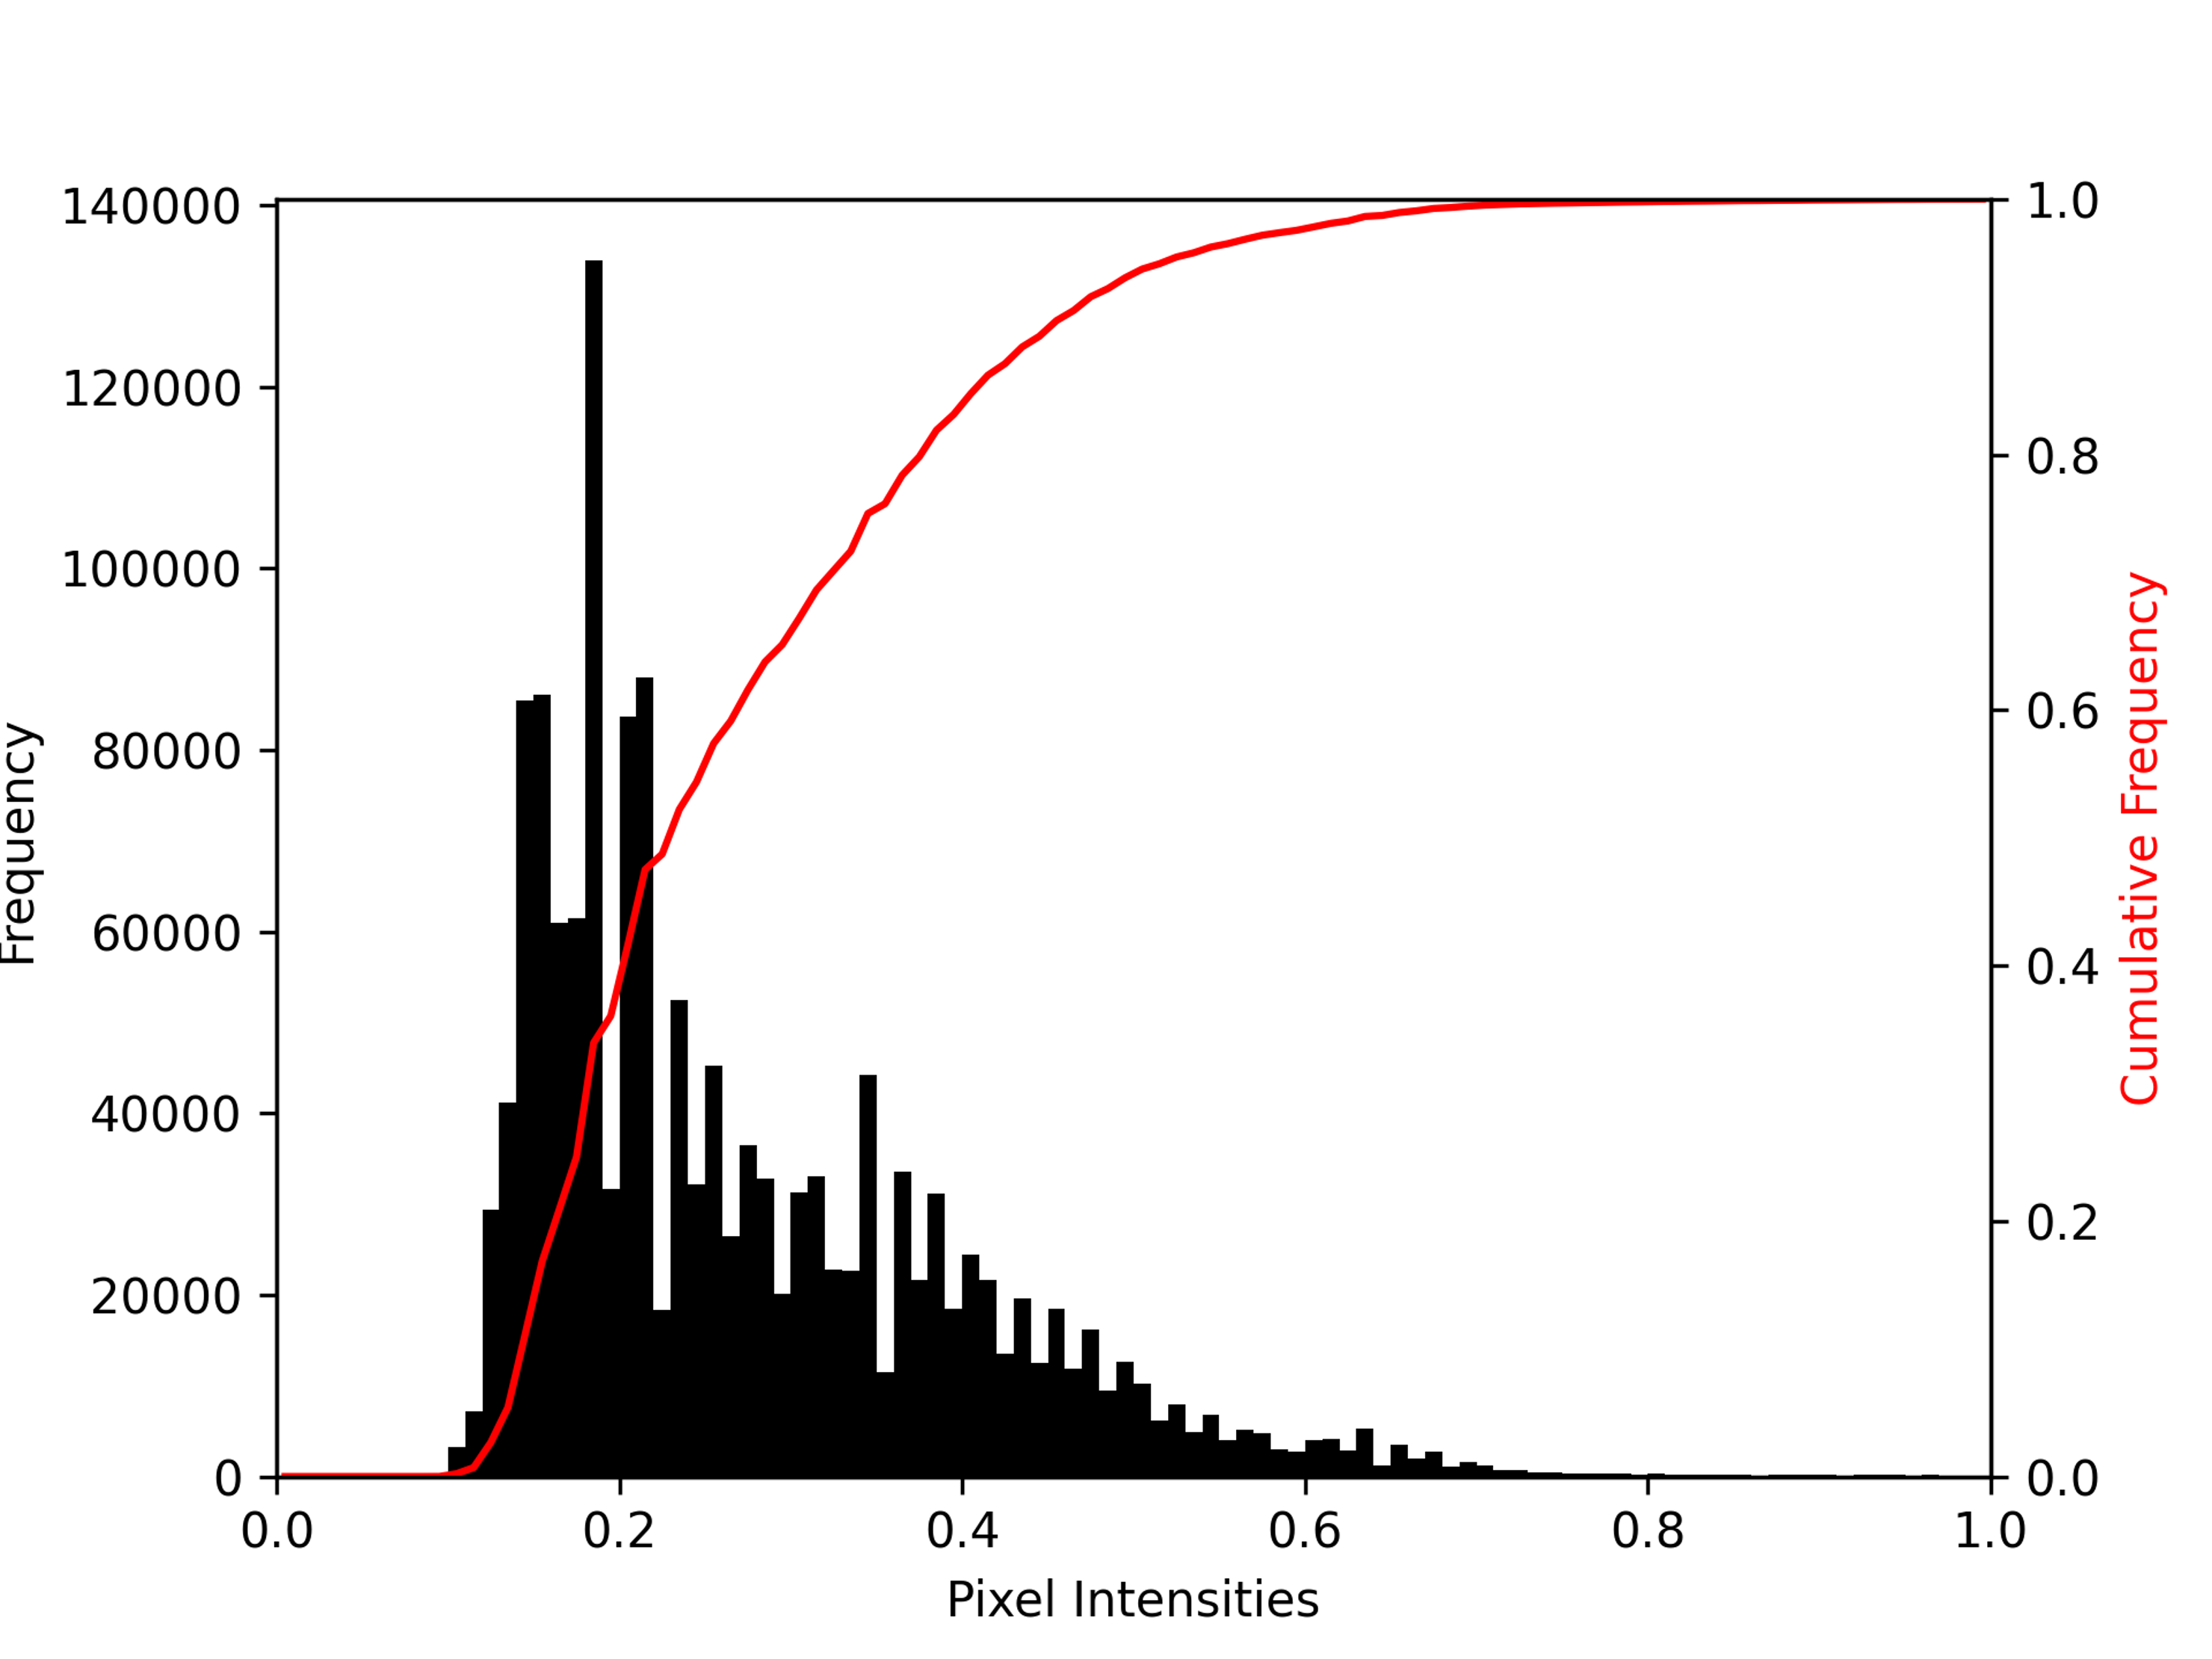
\includegraphics[width=0.8\textwidth]{fig_17.png}
    \caption{Histogram and CDF from UTC: 22/11/2021 14:16:52.}
\end{figure}
\FloatBarrier
The contrast of the images tends to be on the lower side. Box plots for each sequence (as shown in Figure 2.15) confirm the visual observations. Pixel data, up to the third quartile, is concentrated in low-to-medium intensities, resulting in dark images. However, some data points are scattered across higher intensities. Additionally, the median values in the box plots indicate variations in brightness levels within each sequence. Pixel Intensity histograms (see Figure 2.16), plotted with 100 bins, show a positive skewness across all image sequences, reflecting the fewer lighter intensities. The cumulative distribution function (CDF), plotted alongside the histogram, illustrates the rate of increase in intensities across the lower-to-medium intensity range.

After analysing the image data in the spatial domain, the fourier transform was computed to obtain details about the frequency domain, revealing cloudy features in higher frequencies (see Figure 2.17). 
\FloatBarrier
\begin{figure}[h!]
    \centering
    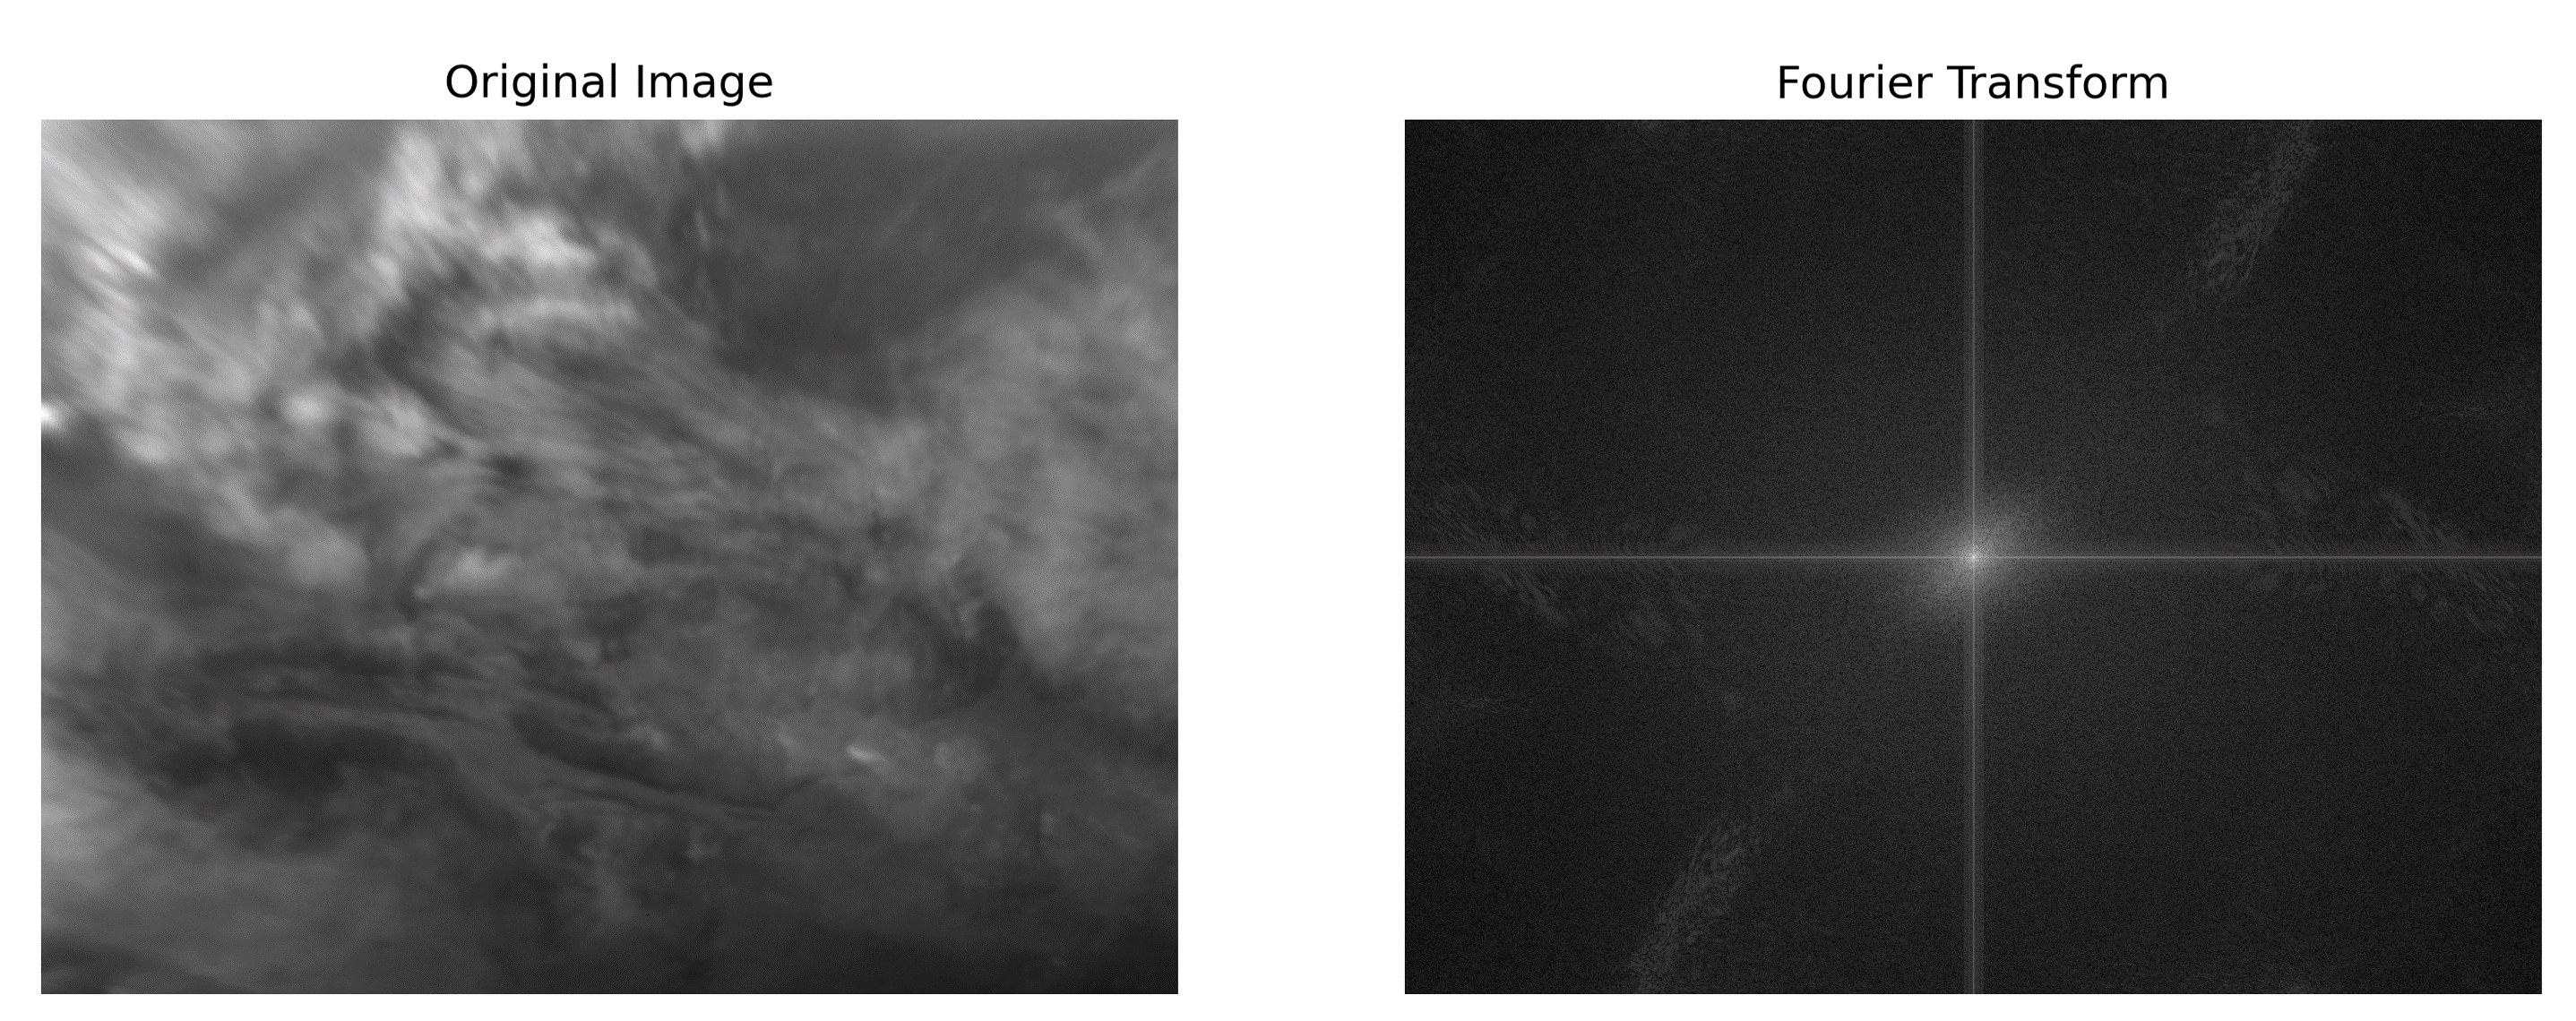
\includegraphics[width=1\textwidth]{fig_18.png}
    \caption{Magnitude spectrum of image from UTC: 23/10/2023 05:40:13.}
\end{figure}
\FloatBarrier
To investigate these features, a high-pass filter with a cut-off radius of 40 pixels was applied (see Figure 2.18), which removes lower-frequency components, highlighting the higher-frequency details. Subsequently, the square-root of the pixels was computed to enhance the image's brightness.
\FloatBarrier
\begin{figure}[h!]
    \centering
    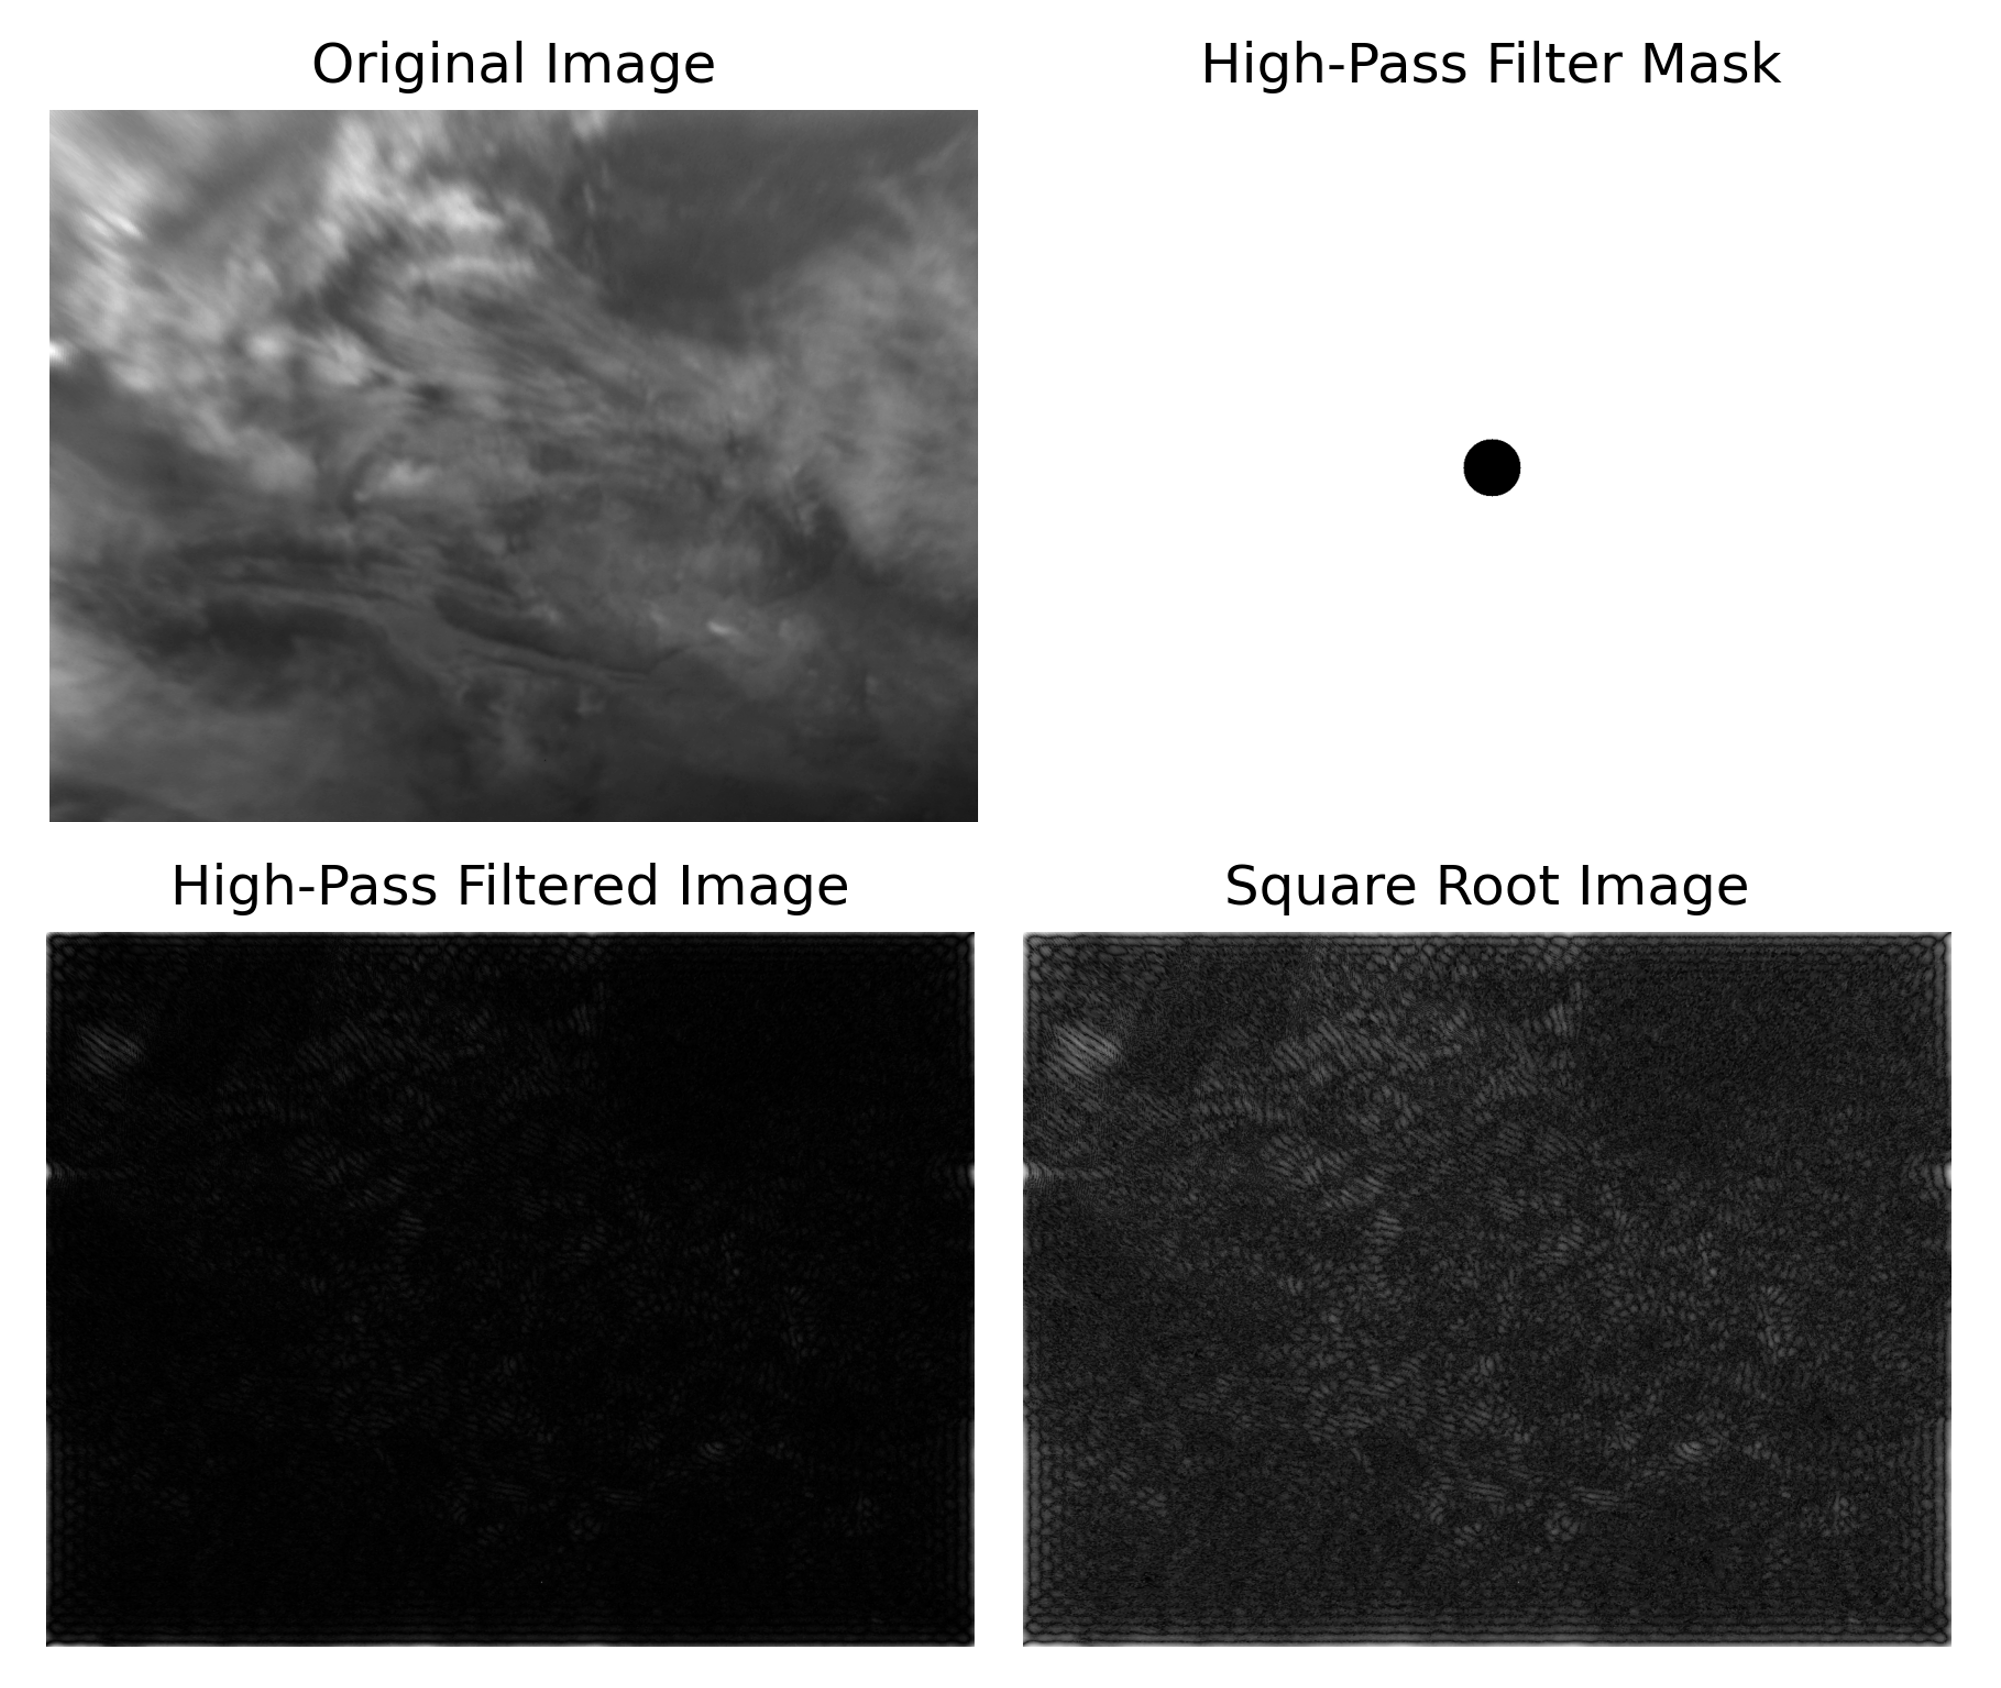
\includegraphics[width=1\textwidth]{fig_19.png}
    \caption{UTC: 23/10/2023 05:40:13 - overview of original image, high-pass filter mask, high-pass filtered image and square root image. The pixels of the high-pass filtered image were transformed using the square root to enhance contrast and improve visualization.}
\end{figure}
\FloatBarrier
The results indicate the presence of atmospheric waves. Increasing the cut-off radius in the high-pass filter highlights shorter wavelengths, while a lower cut-off radius brings out longer wavelengths. However, a cut-off radius that is too large, is not effective since the upper limit of the wavelength is constrained and a cut-off radius that is too small doesn't capture meaningful results either, possibly due to pixel resolution (see Figure A.1).
